\scanpage{138}
\mspage{68}
\unsure{évidemment} l'image inverse de $D^{*}_{\unsure{\widetilde{d'}_*}}$, c'est aussi l'image inverse de $\Theta^{(d)*}_{\unsure{d_*}}$.

\deleted{\unsure{Comme on a encore les diagrammes}}

Finalement, on est ramené à la

\uline{Situation clef}\quad $\unsure{Y}$ espace analytique lisse, muni d'un diviseur $\Theta$ à croisements normaux, $D''$ et $D'$ deux espaces analytiques \inserted{lisses} et
\[
(230)\qquad D''^{*}\longrightarrow D'\longrightarrow \unsure{Y}
\]
des morphismes, qui sont \uline{localement} des immersions \deleted{\unsure{de}}, on suppose $D''^{*}$ de codim $d_0$, $D'$ de codim $d_1$ dans $Y$, donc $D''^{*}$ de codim $d=d_1-d_0$ dans $D'$, et que $D'\to Y$ se factorise par $\Theta^{(d_1)}$ (squelette de dim $d_1$ de $\Theta$), \deleted{\unsure{et} $d_1>d_0\geq0$} et $D''^{*}\to Y$ se factorise par $\Theta^{(d_0)*}$ (squelette \deleted{\unsure{de dim}} de codim $d_0$ de $\Theta$). \inserted{On désigne par $D''^{*}$ et $D'^{*}$ les images inverses de $\Theta^{(d_0)*}$ et $\Theta^{(d_1)*}$.} On a donc $\Theta$ une structure \unsure{constante} le long de $D''^{*}$ : savoir réunion locale de $d_0$ branches non singulières \deleted{\unsure{qui}} de codim $d_0$ qui se coupent suivant $D''$). On considère les ``fibrés principaux multinormaux'' $P_{D''},P_{D'}$, associés aux immersions locales $D''\to Y$, $D'\to Y$, et les groupoïdes

\margin{$d_1\geq d_0\geq0$ (cas $d_0=0$ non \unsure{exclus}, mais trivial)}
\margin{Cela signifie qu'on a un \unsure{diagramme} commutatif
\diagram{\begin{tikzcd}[ampersand replacement=\&,column sep=large]
D''^{*}\arrow[r]\arrow[d,"\mathrm{ét}"] \& D'\arrow[d,"\mathrm{ét}"]\arrow[dr,dashed] \& \\
D^{*}_{d_0,d_1}\arrow[r] \& D_{d_1}\arrow[r] \& D_0=Y
\end{tikzcd}}
\unsure{can.}\quad\unsure{can.}}
\margin{137}

\scanpage{139}
\margin{\deleted{(où $D'^{*}$ est l'image inv. de $\Theta^{(d_1)*}$)}}
fondamentaux $\Pi_1P_{D''^{*}},\Pi_1P_{D'^{*}}$, Cette fois, on a un morphisme canonique (dit ``de générisation'')
\[
(231)\qquad \boxed{\Pi_1P_{D''^{*}}\xrightarrow{\gamma_{D'',D'}}\Pi_1P_{D'^{*}}}.
\]
\deleted{\unsure{compatible avec les opérations de}}

On donnera la \inserted{\unsure{principe de|principale}} construction de ce morphisme, et ses principales propriétés formelles, dans la suite. Notons tout de suite qu'on a un morphisme trivial, déduit de l'inclusion
\[
\deleted{\unsure{P_{D'^{*}}=P_{D'}\vert D'^{*}\longrightarrow P_{D'}}}
\]
\[
P_{D'^{*}}=P_{D'}\vert D'^{*}\lhook\joinrel\longrightarrow P_{D'}
\]
\[
(232)\qquad\Pi_1P_{D'^{*}}\longrightarrow\Pi_1P_{D'}
\]
donc le composé de (231) et (232) fournit
\[
(233)\qquad\Pi_1P_{D'^{*}}\longrightarrow\Pi_1P_{D'},
\]
qui, lui, est de nature entièrement trivial, car on a en effet un morphisme évident $P_{D'}\longrightarrow P_{D''}$. En fait,
\margin{138}

\scanpage{140}
\mspage{69}
on doit avoir commutativité dans
\[
(234)\qquad
\diagram{\begin{tikzcd}[ampersand replacement=\&]
\Pi_1P_{D''^{*}}\arrow[r,"\gamma_{D'',D'}"]\arrow[d,"i_{D''}"'] \& \Pi_1P_{D'^{*}}\arrow[d,"i_{D'}"]\\
\Pi_1P_{D''}\arrow[r] \& \Pi_1P_{D'}
\end{tikzcd}}.
\]
On fera bien attention \unsure{entre|à} la différence entre la flèche composée $i_{D'}\gamma_{D'',D'}$, de nature triviale, et la flèche $\gamma_{D'',D'}$, qui ne correspond à aucun morphisme $P_{D''^{*}}\mathbin{-}P_{D'^{*}}$ (\uline{NB} l'image de $D''$ dans $D'$ est contenue juste en $D'\setminus D'^{*}$ !).

Le principe de la construction de (231) est le suivant. Pour une immersion locale d'espaces analytiques lisses telle que $D'\longrightarrow Y$ (relative à un diviseur $\Theta$ à croisements normaux sur $Y$, i.e. se factorisant par
\diagram{\begin{tikzcd}[ampersand replacement=\&,column sep=small]
D'\arrow[r,"\text{étale}"] \& \deleted{\unsure{\Theta}}\;D_{\unsure{d_1}}\arrow[r] \& Y=D_0
\end{tikzcd}}), on introduit \deleted{\unsure{le}} (en fait, indépendamment de la donnée de $\Theta$) le ``voisinage tubulaire de $D'$ \deleted{\unsure{p}} dans $Y$'', comme un \uline{germe} d'espace analytique \deleted{\unsure{aut}} autour de $D'$
\margin{139}

\scanpage{141}
p.ex. si l'image de $D'$ dans $Y$ est figurée par
\figure{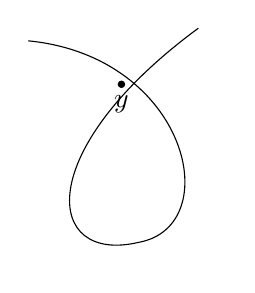
\begin{tikzpicture}[scale=.8]
\draw (-1.45,1.65) .. controls (1.1,1.4) and (1.7,-1.3) .. (.3,-1.55) .. controls (-1.2,-1.9) and (-1.4,-.1) .. (1.25,1.85);
\fill (.03,.96) circle (1.7pt);
\node[below] at (.03,.94) {$\unsure{y}$};
\end{tikzpicture}}, le voisinage tubulaire en question sera figuré \inserted{dans $Y$} par
\figure{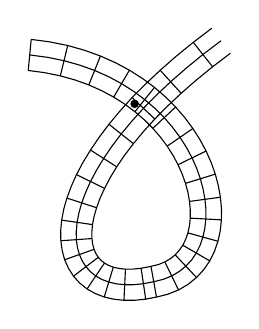
\begin{tikzpicture}[scale=.9,line width=.4pt]
\draw (-1.471,1.431) -- (-1.238,1.400) -- (-1.018,1.355) -- (-0.811,1.297) -- (-0.616,1.227) -- (-0.435,1.146) -- (-0.265,1.055) -- (-0.109,0.956) -- (0.035,0.849) -- (0.167,0.735) -- (0.287,0.615) -- (0.394,0.491) -- (0.490,0.363) -- (0.573,0.232) -- (0.643,0.101) -- (0.702,-0.031) -- (0.748,-0.162) -- (0.783,-0.291) -- (0.805,-0.417) -- (0.816,-0.538) -- (0.816,-0.653) -- (0.804,-0.761) -- (0.782,-0.861) -- (0.751,-0.952) -- (0.710,-1.035) -- (0.661,-1.107) -- (0.603,-1.171) -- (0.535,-1.225) -- (0.457,-1.271) -- (0.366,-1.308) -- (0.261,-1.333) -- (0.250,-1.336) -- (0.122,-1.360) -- (0.006,-1.372) -- (-0.099,-1.373) -- (-0.191,-1.363) -- (-0.271,-1.345) -- (-0.338,-1.319) -- (-0.395,-1.287) -- (-0.443,-1.249) -- (-0.482,-1.205) -- (-0.515,-1.154) -- (-0.542,-1.093) -- (-0.561,-1.022) -- (-0.572,-0.941) -- (-0.573,-0.848) -- (-0.564,-0.744) -- (-0.542,-0.630) -- (-0.506,-0.506) -- (-0.458,-0.373) -- (-0.394,-0.233) -- (-0.316,-0.084) -- (-0.222,0.071) -- (-0.113,0.232) -- (0.013,0.398) -- (0.156,0.570) -- (0.315,0.746) -- (0.492,0.925) -- (0.687,1.109) -- (0.899,1.294) -- (1.131,1.483) -- (1.380,1.673);
\draw (-1.450,1.650) -- (-1.202,1.617) -- (-0.966,1.569) -- (-0.744,1.506) -- (-0.534,1.431) -- (-0.338,1.344) -- (-0.154,1.245) -- (0.016,1.137) -- (0.173,1.020) -- (0.317,0.896) -- (0.448,0.765) -- (0.566,0.628) -- (0.671,0.488) -- (0.762,0.344) -- (0.841,0.197) -- (0.906,0.050) -- (0.958,-0.097) -- (0.997,-0.244) -- (1.023,-0.388) -- (1.036,-0.528) -- (1.035,-0.665) -- (1.021,-0.796) -- (0.994,-0.920) -- (0.954,-1.037) -- (0.900,-1.145) -- (0.834,-1.244) -- (0.753,-1.331) -- (0.660,-1.406) -- (0.553,-1.469) -- (0.433,-1.517) -- (0.300,-1.550) -- (0.300,-1.550) -- (0.154,-1.578) -- (0.018,-1.592) -- (-0.109,-1.593) -- (-0.227,-1.580) -- (-0.334,-1.555) -- (-0.432,-1.518) -- (-0.518,-1.469) -- (-0.593,-1.409) -- (-0.657,-1.338) -- (-0.709,-1.257) -- (-0.749,-1.166) -- (-0.777,-1.066) -- (-0.792,-0.957) -- (-0.793,-0.839) -- (-0.781,-0.712) -- (-0.756,-0.579) -- (-0.716,-0.438) -- (-0.661,-0.290) -- (-0.592,-0.136) -- (-0.507,0.024) -- (-0.407,0.189) -- (-0.291,0.360) -- (-0.159,0.535) -- (-0.010,0.714) -- (0.155,0.897) -- (0.338,1.083) -- (0.539,1.272) -- (0.758,1.463) -- (0.994,1.656) -- (1.250,1.850);
\draw (-1.429,1.869) -- (-1.165,1.834) -- (-0.914,1.783) -- (-0.677,1.716) -- (-0.452,1.635) -- (-0.241,1.541) -- (-0.043,1.435) -- (0.141,1.318) -- (0.311,1.192) -- (0.467,1.057) -- (0.609,0.915) -- (0.738,0.766) -- (0.852,0.612) -- (0.952,0.455) -- (1.039,0.294) -- (1.111,0.131) -- (1.169,-0.032) -- (1.212,-0.196) -- (1.241,-0.358) -- (1.256,-0.519) -- (1.255,-0.677) -- (1.239,-0.831) -- (1.206,-0.979) -- (1.157,-1.122) -- (1.091,-1.256) -- (1.006,-1.380) -- (0.904,-1.491) -- (0.785,-1.587) -- (0.650,-1.666) -- (0.501,-1.726) -- (0.339,-1.767) -- (0.350,-1.764) -- (0.187,-1.796) -- (0.030,-1.812) -- (-0.120,-1.812) -- (-0.263,-1.797) -- (-0.398,-1.766) -- (-0.525,-1.717) -- (-0.641,-1.652) -- (-0.744,-1.570) -- (-0.832,-1.472) -- (-0.903,-1.361) -- (-0.957,-1.240) -- (-0.992,-1.110) -- (-1.011,-0.972) -- (-1.013,-0.829) -- (-0.999,-0.681) -- (-0.970,-0.528) -- (-0.925,-0.370) -- (-0.865,-0.207) -- (-0.790,-0.039) -- (-0.699,0.133) -- (-0.592,0.308) -- (-0.470,0.488) -- (-0.332,0.672) -- (-0.177,0.858) -- (-0.005,1.048) -- (0.185,1.240) -- (0.391,1.434) -- (0.616,1.631) -- (0.858,1.828) -- (1.120,2.027);
\draw (-1.471,1.431) -- (-1.429,1.869);
\draw (-1.018,1.355) -- (-0.914,1.783);
\draw (-0.616,1.227) -- (-0.452,1.635);
\draw (-0.265,1.055) -- (-0.043,1.435);
\draw (0.035,0.849) -- (0.311,1.192);
\draw (0.287,0.615) -- (0.609,0.915);
\draw (0.490,0.363) -- (0.852,0.612);
\draw (0.643,0.101) -- (1.039,0.294);
\draw (0.748,-0.162) -- (1.169,-0.032);
\draw (0.805,-0.417) -- (1.241,-0.358);
\draw (0.816,-0.653) -- (1.255,-0.677);
\draw (0.782,-0.861) -- (1.206,-0.979);
\draw (0.710,-1.035) -- (1.091,-1.256);
\draw (0.603,-1.171) -- (0.904,-1.491);
\draw (0.457,-1.271) -- (0.650,-1.666);
\draw (0.261,-1.333) -- (0.339,-1.767);
\draw (0.122,-1.360) -- (0.187,-1.796);
\draw (-0.099,-1.373) -- (-0.120,-1.812);
\draw (-0.271,-1.345) -- (-0.398,-1.766);
\draw (-0.395,-1.287) -- (-0.641,-1.652);
\draw (-0.482,-1.205) -- (-0.832,-1.472);
\draw (-0.542,-1.093) -- (-0.957,-1.240);
\draw (-0.572,-0.941) -- (-1.011,-0.972);
\draw (-0.564,-0.744) -- (-0.999,-0.681);
\draw (-0.506,-0.506) -- (-0.925,-0.370);
\draw (-0.394,-0.233) -- (-0.790,-0.039);
\draw (-0.222,0.071) -- (-0.592,0.308);
\draw (0.013,0.398) -- (-0.332,0.672);
\draw (0.315,0.746) -- (-0.005,1.048);
\draw (0.687,1.109) -- (0.391,1.434);
\draw (1.131,1.483) -- (0.858,1.828);\fill (.03,.96) circle (1.7pt);\end{tikzpicture}}, et hors de $Y$ par
\figure{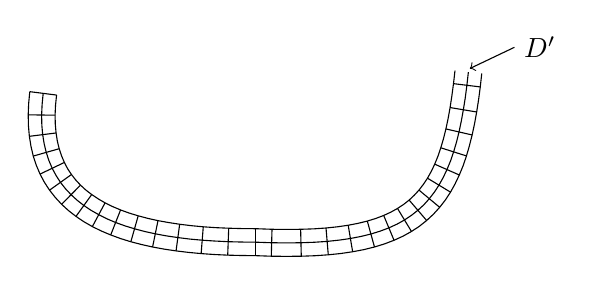
\begin{tikzpicture}[scale=.9,line width=.4pt]
\draw (-3.189,1.224) -- (-3.205,1.057) -- (-3.211,0.897) -- (-3.208,0.742) -- (-3.195,0.594) -- (-3.172,0.452) -- (-3.140,0.315) -- (-3.097,0.185) -- (-3.044,0.061) -- (-2.982,-0.056) -- (-2.910,-0.166) -- (-2.829,-0.269) -- (-2.740,-0.365) -- (-2.643,-0.454) -- (-2.537,-0.536) -- (-2.425,-0.612) -- (-2.306,-0.680) -- (-2.180,-0.742) -- (-2.047,-0.798) -- (-1.908,-0.849) -- (-1.763,-0.894) -- (-1.612,-0.933) -- (-1.456,-0.968) -- (-1.293,-0.998) -- (-1.125,-1.023) -- (-0.951,-1.044) -- (-0.771,-1.061) -- (-0.586,-1.074) -- (-0.396,-1.083) -- (-0.201,-1.088) -- (0.000,-1.090) -- (-0.008,-1.090) -- (0.219,-1.098) -- (0.436,-1.100) -- (0.642,-1.098) -- (0.838,-1.091) -- (1.023,-1.078) -- (1.199,-1.060) -- (1.367,-1.035) -- (1.525,-1.005) -- (1.675,-0.968) -- (1.817,-0.924) -- (1.951,-0.873) -- (2.078,-0.815) -- (2.197,-0.749) -- (2.308,-0.676) -- (2.411,-0.594) -- (2.507,-0.505) -- (2.595,-0.408) -- (2.675,-0.305) -- (2.748,-0.194) -- (2.813,-0.076) -- (2.872,0.048) -- (2.926,0.179) -- (2.973,0.317) -- (3.015,0.462) -- (3.053,0.613) -- (3.087,0.771) -- (3.117,0.937) -- (3.144,1.110) -- (3.168,1.291) -- (3.189,1.480);
\draw (-3.000,1.200) -- (-3.015,1.044) -- (-3.022,0.894) -- (-3.019,0.752) -- (-3.007,0.617) -- (-2.986,0.489) -- (-2.957,0.367) -- (-2.919,0.252) -- (-2.873,0.143) -- (-2.818,0.041) -- (-2.756,-0.056) -- (-2.685,-0.146) -- (-2.606,-0.230) -- (-2.520,-0.309) -- (-2.426,-0.382) -- (-2.325,-0.450) -- (-2.216,-0.512) -- (-2.101,-0.570) -- (-1.978,-0.622) -- (-1.848,-0.669) -- (-1.711,-0.711) -- (-1.568,-0.749) -- (-1.418,-0.782) -- (-1.262,-0.811) -- (-1.099,-0.835) -- (-0.931,-0.856) -- (-0.756,-0.872) -- (-0.575,-0.884) -- (-0.389,-0.893) -- (-0.197,-0.898) -- (0.000,-0.900) -- (0.000,-0.900) -- (0.224,-0.908) -- (0.436,-0.910) -- (0.637,-0.908) -- (0.828,-0.901) -- (1.007,-0.889) -- (1.176,-0.871) -- (1.335,-0.848) -- (1.484,-0.819) -- (1.624,-0.785) -- (1.756,-0.744) -- (1.878,-0.698) -- (1.992,-0.646) -- (2.098,-0.587) -- (2.196,-0.522) -- (2.287,-0.450) -- (2.372,-0.372) -- (2.449,-0.286) -- (2.520,-0.194) -- (2.585,-0.095) -- (2.644,0.011) -- (2.698,0.125) -- (2.748,0.246) -- (2.792,0.375) -- (2.832,0.511) -- (2.868,0.656) -- (2.900,0.808) -- (2.929,0.968) -- (2.956,1.137) -- (2.979,1.314) -- (3.000,1.500);
\draw (-2.811,1.176) -- (-2.826,1.030) -- (-2.832,0.892) -- (-2.829,0.763) -- (-2.818,0.641) -- (-2.800,0.526) -- (-2.774,0.419) -- (-2.741,0.319) -- (-2.701,0.225) -- (-2.655,0.137) -- (-2.601,0.055) -- (-2.540,-0.023) -- (-2.473,-0.095) -- (-2.398,-0.164) -- (-2.315,-0.228) -- (-2.225,-0.288) -- (-2.127,-0.345) -- (-2.021,-0.397) -- (-1.908,-0.445) -- (-1.787,-0.489) -- (-1.659,-0.528) -- (-1.523,-0.564) -- (-1.380,-0.596) -- (-1.230,-0.623) -- (-1.074,-0.647) -- (-0.910,-0.667) -- (-0.741,-0.683) -- (-0.564,-0.695) -- (-0.382,-0.703) -- (-0.194,-0.708) -- (0.000,-0.710) -- (0.008,-0.710) -- (0.229,-0.718) -- (0.437,-0.720) -- (0.633,-0.718) -- (0.818,-0.712) -- (0.991,-0.700) -- (1.153,-0.683) -- (1.304,-0.661) -- (1.444,-0.634) -- (1.574,-0.602) -- (1.694,-0.565) -- (1.805,-0.523) -- (1.906,-0.476) -- (2.000,-0.424) -- (2.085,-0.368) -- (2.164,-0.306) -- (2.236,-0.238) -- (2.303,-0.165) -- (2.365,-0.084) -- (2.423,0.003) -- (2.476,0.098) -- (2.525,0.201) -- (2.570,0.312) -- (2.611,0.432) -- (2.649,0.561) -- (2.683,0.698) -- (2.714,0.844) -- (2.742,1.000) -- (2.767,1.164) -- (2.790,1.337) -- (2.811,1.520);
\draw (-3.189,1.224) -- (-2.811,1.176);
\draw (-3.211,0.897) -- (-2.832,0.892);
\draw (-3.195,0.594) -- (-2.818,0.641);
\draw (-3.140,0.315) -- (-2.774,0.419);
\draw (-3.044,0.061) -- (-2.701,0.225);
\draw (-2.910,-0.166) -- (-2.601,0.055);
\draw (-2.740,-0.365) -- (-2.473,-0.095);
\draw (-2.537,-0.536) -- (-2.315,-0.228);
\draw (-2.306,-0.680) -- (-2.127,-0.345);
\draw (-2.047,-0.798) -- (-1.908,-0.445);
\draw (-1.763,-0.894) -- (-1.659,-0.528);
\draw (-1.456,-0.968) -- (-1.380,-0.596);
\draw (-1.125,-1.023) -- (-1.074,-0.647);
\draw (-0.771,-1.061) -- (-0.741,-0.683);
\draw (-0.396,-1.083) -- (-0.382,-0.703);
\draw (0.000,-1.090) -- (0.000,-0.710);
\draw (0.219,-1.098) -- (0.229,-0.718);
\draw (0.642,-1.098) -- (0.633,-0.718);
\draw (1.023,-1.078) -- (0.991,-0.700);
\draw (1.367,-1.035) -- (1.304,-0.661);
\draw (1.675,-0.968) -- (1.574,-0.602);
\draw (1.951,-0.873) -- (1.805,-0.523);
\draw (2.197,-0.749) -- (2.000,-0.424);
\draw (2.411,-0.594) -- (2.164,-0.306);
\draw (2.595,-0.408) -- (2.303,-0.165);
\draw (2.748,-0.194) -- (2.423,0.003);
\draw (2.872,0.048) -- (2.525,0.201);
\draw (2.973,0.317) -- (2.611,0.432);
\draw (3.053,0.613) -- (2.683,0.698);
\draw (3.117,0.937) -- (2.742,1.000);
\draw (3.168,1.291) -- (2.790,1.337);\draw[<-] (3.02,1.55)--(3.65,1.85) node[right] {$D'$};\end{tikzpicture}}.

Cette construction est possible dans le cadre (p.ex.) des \inserted{\unsure{paires (loc. fer.) de}} variétés différentiables, \inserted{paracompactes} en tant que germe de variété autour de $D'$ (défini à iso unique près ?...). Dans le cadre des \uline{multiplicités} \deleted{topologiques}, \inserted{\unsure{diff. (voire topologiques)},} on peut encore définir ce voisinage comme un germe de \deleted{topos}, \inserted{multiplicité diff.} par descente à partir d'une situation d'\deleted{espaces analytiques} \inserted{variétés diff. (ou top.)} paracompactes. On peut aussi, me semble-t-il, donner
\margin{140}

\scanpage{142}
\mspage{70}
une définition directe, \deleted{valable} dans un style encore plus topologique, valable chaque fois au moins (sauf erreur) où on a une immersion locale de \uline{topos}. On va désigner par $\mathcal V_{D',Y}$ le ``voisinage tubulaire'' défini \inserted{en fait} par une immersion \deleted{\unsure{top}} locale topologique. Il a des propriétés de fonctorialité telles, que l'on tire, \deleted{\unsure{dans}} partant d'une situation \deleted{\unsure{de deux}} d'un composé d'immersions locales $D''\mathbin{-}D'\mathbin{-}Y$, \deleted{\unsure{d'un}} un diagramme \unsure{comm.} canonique
\[
(235)\quad\deleted{\unsure{\mathcal V_{D'',Y}}}\quad
\diagram{\begin{tikzcd}[ampersand replacement=\&]
D''\arrow[r,dash]\arrow[d,hook] \& D'\arrow[d,hook] \& \\
\mathcal V_{D'',Y}\arrow[r,"\substack{\mathrm{imm.}\\\mathrm{locale}}"'] \& \mathcal V_{D',Y}\arrow[r,"\substack{\mathrm{imm.}\\\mathrm{locale}}"'] \& Y
\end{tikzcd}}
\]
\margin{\deleted{\unsure{(234)}}
\figure{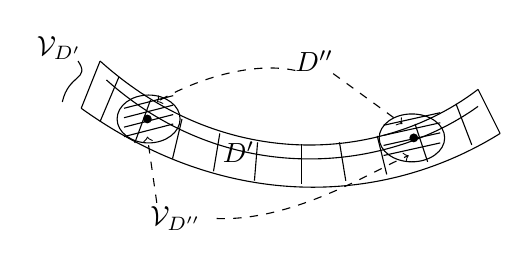
\begin{tikzpicture}[scale=.8]
\draw (-3,1.1) .. controls (-1,-.7) and (1.5,-.5) .. (3,.65);
\draw (-3.3,.35) .. controls (-1,-1.3) and (1.5,-1.2) .. (3.35,-.05);
\draw (-2.9,.8) .. controls (-1,-.9) and (1.5,-.7) .. (3,.38);
\draw (-3,1.1)--(-3.3,.35);\draw (3,.65)--(3.35,-.05);
\draw (-2.7,.85)--(-3,.14);\draw (-2.2,.48)--(-2.45,-.2);
\draw (-1.7,.18)--(-1.85,-.45);\draw (-1.1,-.05)--(-1.2,-.65);
\draw (-.5,-.19)--(-.55,-.8);\draw (.2,-.22)--(.2,-.85);
\draw (.8,-.19)--(.9,-.8);\draw (1.4,-.09)--(1.55,-.7);
\draw (2,.1)--(2.2,-.5);\draw (2.65,.42)--(2.9,-.23);
\draw (-2.23,.18) ellipse (.5 and .38);\draw (1.95,-.12) ellipse (.52 and .38);
\foreach \y in {-.1,.05,.2,.35} {\draw (-2.62,\y)--(-1.84,\y+.2);}
\foreach \y in {-.4,-.24,-.08,.08} {\draw (1.5,\y)--(2.4,\y+.2);}
\fill (-2.25,.18) circle(2pt);\fill (1.98,-.12) circle(2pt);
\node at (-.8,-.35) {$D'$};\node at (.4,1.1) {$D''$};
\draw[->,dashed] (.1,.95).. controls (-.6,1.1) and (-1.5,.8)..(-2.1,.45);
\draw[->,dashed] (.7,.9)--(1.8,.1);
\node at (-3.65,1.3) {$\mathcal V_{D'}$};\draw (-3.35,1.1) .. controls (-3.15,.8) and (-3.5,.9)..(-3.6,.45);
\node at (-1.8,-1.4) {$\mathcal V_{D''}$};
\draw[dashed,->] (-2.1,-1.15)--(-2.25,-.1);
\draw[dashed,->] (-1.15,-1.4).. controls (.1,-1.45) and (1.4,-.6)..(1.9,-.4);
\end{tikzpicture}}}

\deleted{\unsure{Donc}} Pour l'instant, on n'a pas utilisé le diviseur $\Theta$ à croisements normaux dans $Y$ définissant \inserted{l'ouvert} $Y^{*}=Y\setminus\Theta$. \unsure{Nou|N.} Nous considérons maintenant l'image inverse de $Y^{*}$ dans $\mathcal V_{D',Y}$ et $\mathcal V_{D'',Y}$, soient $\mathcal V^{*}_{D',Y}$ et $\mathcal V^{*}_{D'',Y}$, s'insérant dans un diagramme
\margin{141}

\scanpage{143}
\[
(236)\quad
\diagram{\begin{tikzcd}[ampersand replacement=\&,column sep=large]
\deleted{\unsure{D^{*}}}\;\mathcal V^{*}_{D'',Y}\arrow[r]\arrow[d,equal] \& \mathcal V^{*}_{D',Y}\arrow[r]\arrow[d,equal] \& Y\\
\mathcal V_{D'',Y}\setminus\underbrace{\Theta_{D'',Y}}_{\substack{\text{image inverse}\\\text{de }\Theta\text{ sur }\mathcal V_{D'',Y}}} \& \mathcal V_{D',Y}\setminus\Theta_{D',Y} \&
\end{tikzcd}}
\]
\margin{\uline{NB} $\mathcal V^{*}_{D'',Y}$ a la structure du complémentaire d'un diviseur à croisements normaux \inserted{$\Theta''$}, dans un voisinage tubulaire de $\Theta''^{(d_0)*}$ --- et analogue pour $\mathcal V^{*}_{D',Y}$}
\figure{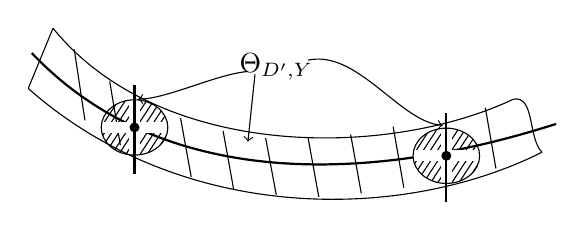
\begin{tikzpicture}[scale=.9]
\draw (-3.3,1.25) .. controls (-1.8,-.6) and (1.4,-.6) .. (3.2,.25);
\draw (-3.65,.4) .. controls (-1.5,-1.5) and (1.6,-1.5) .. (3.6,-.5);
\draw[line width=.8pt] (-3.6,.9) .. controls (-1.7,-1.1) and (1.3,-.9) .. (3.8,-.1);
\draw (-3.3,1.25)--(-3.65,.4);\draw (3.2,.25)..controls(3.5,.3)and(3.4,-.3)..(3.6,-.5);
\foreach \x/\a/\b in {-3/.95/-.05,-2.5/.5/-.4,-1.5/-.02/-.85,-.9/-.2/-1.03,-.3/-.3/-1.1,.3/-.3/-1.13,.9/-.25/-1.08,1.5/-.14/-1,2.8/.13/-.73}{\draw (\x,\a)--(\x+.15,\b);}
\foreach \x/\y in {-2.15/-.15,2.25/-.55}{
\begin{scope}\clip (\x,\y) ellipse (.47 and .39);
\foreach \s in {-1,-.9,...,1}{\draw (\x+\s,\y-.5)--(\x+\s+.65,\y+.5);}
\draw[white,line width=4pt] (\x-.5,\y)--(\x+.5,\y);\draw[white,line width=4pt] (\x,\y-.5)--(\x,\y+.5);
\end{scope}
\draw (\x,\y) ellipse (.47 and .39);\draw[line width=.8pt] (\x,\y-.65)--(\x,\y+.6);\fill (\x,\y) circle(2pt);
}
\node at (-.15,.7) {$\Theta_{D',Y}$};
\draw[->] (-.55,.64)..controls(-1,.6)and(-1.7,.25)..(-2.1,.25);
\draw[->] (-.45,.6)--(-.55,-.35);
\draw[->] (.3,.8)..controls(1,.95)and(1.6,-.08)..(2.2,-.12);
\end{tikzpicture}}

Nous pouvons maintenant définir
\[
(237)\qquad\Pi_1\mathcal V^{*}_{D'',Y}\longrightarrow\Pi_1\mathcal V^{*}_{D',Y}
\]
en définissant les groupoïdes fondamentaux non pas par \inserted{points de} \deleted{base}/\unsure{classes} de chemins, mais par revêtements et isomorphismes entre tels...

C'est en définitive cela, \unsure{l'horreur des|l'heure des} \unsure{normalisations} --- nous pouvons les définir chaque fois qu'on se donne des imm. locales $D''\longrightarrow D'\mathbin{-}Y$
\margin{142}

\scanpage{144}
\mspage{71}
(de topos simplement, si on veut...) et un ouvert $Y^{*}$ de $Y$ [plus génér. un objet du topos \deleted{en question} $Y$, pas la peine \unsure{même} que ce soit un ss-objet de l'objet final, qui dans le cas d'un tel ss-objet, i.e. \unsure{dire} $Y^{*}$ est un ouvert du topos en question) sans supposer que $D'\to Y$ se factorise par $Y\setminus Y^{*}$]. Et on a des propriétés de transitivité tt à fait évidentes pour un composé
\[
(238)\qquad D'''\longrightarrow D''\mathbin{-}D'\longrightarrow Y.
\]
L'hypothèse ``croisements normaux'' va nous servir à expliciter les groupoïdes $\Pi_1\mathcal V^{*}_{D',Y}$, $\Pi_1\mathcal V^{*}_{D'',Y}$ en termes plus simples, comme canoniquement équivalents à $\Pi_1P_{D'^{*}},\Pi_1P_{D''^{*}}$. Donc il faut encore expliciter les \inserted{\uline{\unsure{isom.}} \unsure{(can.)}}

\uline{Théorème}\quad Soit $Y$ un espace analytique complexe, $\Theta$ un diviseur à croisements normaux de $\unsure{Y}$, $D'\longrightarrow Y\deleted{\unsure{\Theta}}$ une immersion
\margin{quitte à remplacer $Y$ par $\mathcal V_{D',Y}$, \unsure{on peut supposer que} $D'\to Y$ est \unsure{une immersion|une vraie immersion}.}
\margin{143}

\scanpage{145}
\margin{L'indice $d_1$ plus haut devient ici $d_0$.}
\inserted{de codim $d$,} qui se factorise par $\Theta^{(d)}$ (NB il est essentiel pour ce qu'on veut faire qu'on n'exige \uline{pas} que $D'\subset\Theta^{(d)*}$), \deleted{\unsure{on en}} d'où un ``voisinage tubulaire'' $\mathcal V_{D',Y}^{\unsure{\deleted{*}}}$ de $D'$ dans $Y$, et par trace de $Y^{*}=Y\setminus\Theta$ un \deleted{\unsure{un}} germe d'espace analytique $\mathcal V^{*}_{D',Y}$. Alors on a une équivalence de groupoïdes, \uline{\unsure{définie} à \deleted{équivalence} isomorphisme unique près}
\[
(239)\qquad\Pi_1\mathcal V^{*}_{D',Y}\xleftarrow{\sim}\Pi_1P_{D'^{*}}
\]
\uline{Remarque} Le cas le plus simple est celui où $Y$ est de dim $1$, et $d=1$, $D'$ réduit à un pt --- le \deleted{\unsure{cas}} cas peut paraître trivial, néanmoins la question de canonicité de l'équivalence m'a semblé nécessiter un soin certain, et fait l'objet de la longue digression des ``notes \unsure{Marche}'' § 53 n° 50 (p. \unsure{768'|7681} ff). Ici \inserted{(en général)} il devrait être ``assez évident'' de définir \inserted{(de façon non canonique)} un plongement \deleted{topologique} \inserted{\unsure{cl.} $C^{\infty}$} (non analytique !)
\margin{144}

\scanpage{146}
\mspage{72}
\[
(240)\qquad\mathcal V_{D',Y}\unsure{\hookrightarrow|\longleftarrow}\underbrace{\check N_{D',Y}}_{\text{fibré normal de }D'\text{ dans }Y}
\]
\deleted{\unsure{transformant la}} dont le composé avec $Y\longrightarrow\mathcal V_{D',Y}$ soit la section nulle, et qui induise l'application identique sur les \deleted{\unsure{fib}}rés normaux le long de la section nulle. Ça \inserted{devrait} marche en tous cas dans le cas de vrais espaces analytiques paracompacts --- c'est faux par contre dans le cas de multiplicités (Ex. $\deleted{D'=\mathbb E^1_{\mathbb C}\subset Y=\mathbb E^2_{\mathbb C}}$, considérons $\mathbb E^1\subset\mathbb E^2$, avec l'opération du groupe discret $\mathbb Z$, \deleted{\unsure{dont}} le générateur opère par la transvection $\begin{pmatrix}1&\unsure{1|0}\\0&1\end{pmatrix}$, on pose $D'=(\mathbb E^1,\mathbb Z)$, $Y=(\mathbb E^2,\mathbb Z)$ --- la \deleted{fibré} extension des fibrés vectoriels différentiables définie par le plongement $D'\subset\mathcal V_{D',Y}\subset Y$ n'est pas scindable, alors que celle définie par la section nulle d'un fibré l'est...). Il est assez clair que lorsqu'on dispose d'une telle immersion (et sans condition $\unsure{=|C^{\infty}}$ de différentiabilité) celle-ci est une ``équivalence d'homotopie'', et
\margin{du moins pour des espaces analytiques ordinaires}
\margin{145}

\scanpage{147}
induit donc une équivalence sur les $\Pi_1$. Mais le bât blesse, du fait qu'on n'a pas de canonicité --- sans compter la nécessité d'hypothèses \inserted{restrictives} gênantes. \deleted{\unsure{Pour trouver quelque chose de canonique}}
\diagram{\begin{tikzcd}[ampersand replacement=\&]
\deleted{\Pi_1^{\unsure{\mathrm{arcs}|\mathrm{accès}}}P_{D'^{*}}}\arrow[r]\arrow[d,"\deleted{\sim}"'] \& \deleted{\Pi_1^{\unsure{\mathrm{rev}}}\mathcal V_{D',Y}}\\
\deleted{\Pi_1^{\unsure{\mathrm{rev}}}P_{D'^{*}}} \& \deleted{\uline{NB}\;\Pi_1^{\unsure{\mathrm{arcs}|\mathrm{accès}}}\mathcal V}
\end{tikzcd}}
\margin{Mais on peut dire qu'on a $\mathcal V^{*}_{D'^{*}}\lhook\joinrel\longrightarrow\mathcal V^{*}_{D'}$ qui induit une équivalence sur les $\Pi_1$, donc il suffit de comparer les $\Pi_1$ des $\mathcal V^{*}_{D'^{*}}$ et $P_{D'^{*}}$, \unsure{en oubliant les généralités précédentes}.}

On a oublié de préciser d'ailleurs, en relation avec le diviseur $\Theta$, qu'on veut que l'é\deleted{\unsure{isom.}}\inserted{plongement (240)} soit tel que l'image inverse de $P^{\deleted{\unsure{*}}}_{D'^{*}}$, identifié à un ouvert de \inserted{($P_{D'}$, lui $=$ ouvert de)} $\check N_{D',Y}$, soit juste $\mathcal V^{*}_{D',Y}$, de sorte qu'on \unsure{trouve} \inserted{bien} \unsure{ainsi|aussi}
\[
\deleted{\Pi_1\mathcal V^{*}_{D',Y}\longrightarrow\Pi_1P_{D'^{*}}}
\]
\[
(241)\qquad\mathcal V^{*}_{D',Y}\longrightarrow P_{D'^{*}}
\]
d'où
\[
(242)\qquad\Pi_1\mathcal V^{*}_{D',Y}\longrightarrow\Pi_1P_{D'^{*}}.
\]
Pour avoir un morphisme de groupoïdes défini de façon plus ``canonique'', et
\margin{146}

\scanpage{148}
\mspage{73}
sans hyp. superflues, \unsure{je} vais plutôt (comme dans Mar p. \unsure{779|769|709} ff) définir une flèche en sens inverse
\[
(243)\qquad\Pi_1^{\mathrm{arcs}}P_{D'^{*}}\longrightarrow\Pi_1^{\mathrm{rev}}\mathcal V^{*}_{D',Y},
\]
où le premier $\Pi_1$ est défini par pts et arcs, et le deuxième (on n'a pas le choix !) est défini en termes de \unsure{rev. + fonc. can.}. Il faut donc généraliser en contexte présent les considérations du loc. cit. Je ne vais pas entrer dans le détail ici --- d'autant moins que je ne vois pas clairement à présent dans quelle mesure le th. \inserted{envisagé} est indispensable --- s'il n'est pas tout aussi commode \deleted{\unsure{et utile}} \inserted{pour la suite} de travailler avec les $\Pi_1\mathcal V^{*}_{D',Y}$ au lieu des $\Pi_1P_{D'^{*}}$ --- en modifiant dans ce sens les définitions des $\widetilde\Pi_{d_0,d_1,\ldots,d_r}$ ; Bien entendu, on aura besoin par la suite que $\widetilde\Pi_{d_0,\ldots,d_r}\mathbin{-}\Pi_{d_0,\ldots,d_r}$ ait une \uline{structure d'extension}, de noyau un quotient de $T_{d_0,\ldots,d_r}$ etc.
\margin{147}

\scanpage{149}
\deleted{Indépendamment de ces faits, \inserted{et sans hyp. spécifique ``crois. normaux''} on voit que $\mathcal V^{*}_{D_1,D_0=X}$ \deleted{peut} s'interprète comme $\mathcal V_{\Theta^{(1)},\unsure{X}}\setminus\Theta^{(1)}$ --- il donne la ``structure à l'infini''}

Reprenons la situation du pt de vue topologique (sans nous \unsure{focuser} sur les $\Pi_1$). Le diviseur $\Theta$ à croisements normaux \inserted{sur $X$} définit une filtration décroissante du \deleted{$X$} analytico-topologique $X$
\[
(244)\qquad\Theta^{(0)}=X\supset\Theta^{(1)}=\Theta\supset\Theta^{(2)}\supset\Theta^{(\unsure{3})}\cdots
\]
On peut définir
\[
D_d=\widetilde{\Theta^{(d)}}\qquad\text{``normalisé topologique'' de }\Theta^{(d)},\text{ dans un sens à préciser }-----,
\]
mais cette définition dépend justement d'hyp ``crois. normaux'' \deleted{\unsure{des}} relativement délicates. Par contre, \deleted{\unsure{D}}
\[
\deleted{D_d^{*}=\Theta^{(d)}\setminus\Theta^{(d-1)}}
\]
\deleted{se définit sans telles hypothèses, donc aussi $\mathcal V_{D_d^{*}}$ et}
\[
\deleted{(245)}\qquad
\diagram{\begin{tikzcd}[ampersand replacement=\&]
\deleted{\mathcal V^{*}_{D_d^{*}}}\arrow[r,hook] \& \deleted{\mathcal V_{D_d^{*}}}
\end{tikzcd}}
\]
\margin{148}

\scanpage{150}
\mspage{74}
Considérons le système $\frac12$ simplicial des
\[
(245)\quad
\diagram{\begin{tikzcd}[ampersand replacement=\&,column sep=small]
\& \mathcal V^{*}_{d_0\ldots d_r}\mathrel{\overset{\mathrm{déf}}=}\mathcal V^{*}_{D_{d_0,\ldots,d_r},X}\arrow[d,hook] \& \text{où }X=D_0\\
D_{d_0,\ldots,d_r}\arrow[r] \& \mathcal V_{d_0,\ldots,d_r}=\mathcal V_{D_{d_0,\ldots,d_r},X} \&
\end{tikzcd}}
\]
\margin{On se \unsure{suppose} $d_0\geq d_1\geq\cdots\geq d_r\unsure{\geq|>}0$.}
les $\mathcal V^{*}_{d_0,\ldots,d_r}$ s'envoient tous \deleted{\unsure{les uns}} \inserted{dans $X^{*}=D_0^{*}=X\setminus\Theta$} et sauf $\mathcal V^{*}_0=X^{*}$, ils \deleted{via $\mathcal V_d^{*}\lhook\joinrel\longrightarrow D$} s'envoient dans $\mathcal V^{*}_{\Theta,X}$.

\uline{Th de recollement}\quad Considérons le \deleted{\unsure{fibré en}} topos \inserted{$\frac12$ simplicial au dessus de $\mathcal V^{*}_{\Theta,X}$, \deleted{\unsure{dont les composantes sont}}} (formé de \unsure{multiplicités} analytiques) formé des $\mathcal V^{*}_{d_0,\ldots,d_r}$ ($d_0\geq d_1\ldots\geq d_r>0$), \deleted{\unsure{Alors on}} soit $\mathcal V^{*}_{\unsure{\bullet}}$, on a un morphisme de la limite inductive de ces topos dans $\mathcal V^{*}_{\Theta,X}$ \inserted{$=X^{*\infty}=D_0^{*\infty}$}, et c'est là une équivalence de topos (a fortiori, \unsure{c'est} une équivalence d'homotopie, et en particulier ça induit un isom. sur les $\pi_0$, et les $\pi_1$ relatifs à des comp. connexes qui se correspondent).
\margin{149}

\scanpage{151}
\uline{Corollaire 1} Fixons un $\delta=\{\delta_0>\delta_1\cdots>\delta_s>0\}$,
considérons $D_{\delta_0,\delta_1,\ldots,\delta_s}=D_\delta$, le diviseur
$\Theta_\delta$ sur $D_\delta$, et $V^*_{\Theta_\delta,D_\delta}=D_\delta^{*\infty}$
(structure à l'infini de $D_\delta^{*\infty}$).

Alors le syst. $\frac12$ simplicial des
\[
\deleted{\unsure{D}}\;V^*_{\underbrace{D_{\underbrace{d_0,\ldots,d_r},\delta_0,\delta_1,\ldots,\delta_s}}_{\text{de degré simp. }r}}
\qquad(\text{pour }d_0>\cdots>d_r>\delta_0
\]
variables) a comme \uline{lim} toposique
la ``structure à l'$\infty$'' $V^*_{\Theta_\delta,D_\delta}=D_\delta^*$.

On applique le th. à $D_\delta,\Theta_\delta\ldots$

\deleted{\uline{Corollaire 2} Supposons que
\diagram{\begin{tikzcd}[ampersand replacement=\&]
V^*_{\Theta,X} \arrow[r,leftrightarrow] \arrow[d,equal,"\mathrm{def}"'] \& X^* \arrow[d,equal] \\
X^{*\infty} \& X\setminus\Theta
\end{tikzcd}}
soit un $1$-\unsure{équivalence} (i.e induise un iso. pour les $\pi_0$, et les $\pi_1$ des comp. conn. correspondantes) alors on a
\[
\deleted{\unsure{\widetilde\Pi_{X,X^*}}}\simeq
\underset{\longrightarrow}{\operatorname{Lim}}\bigl(\deleted{\unsure{\widetilde\Pi_{d_0},\widetilde\Pi}}\bigr)
\quad
\begin{array}{ll}
\widetilde\Pi_{d_0}\deleted{\unsure{\Pi_{d_0}}}&(1\leq d_0\leq3)\\
\widetilde\Pi_{d_0,d_1}&(d_0>d_1\geq
\end{array}
\]
}
\margin{150}

\scanpage{152}
\mspage{75}
\uline{Corollaire 2} On a
\[
(246)\qquad \Pi_1\underbrace{\deleted{X}^{*\infty}}_{=V^*_{\Theta,X}}
\simeq\underset{\longrightarrow}{\operatorname{Lim}}
\left(\vphantom{\widetilde\Pi_{2,1}}\right.
\]
\diagram{\begin{tikzcd}[ampersand replacement=\&,column sep=small]
\&\widetilde\Pi_{2,1}\arrow[dl]\arrow[dr]\&\\
\widetilde\Pi_1\&\&\widetilde\Pi_2
\end{tikzcd}}\[\left.\vphantom{\widetilde\Pi_{2,1}}\right).\]

En effet, une analyse locale facile (du type ``th. de pureté'') montre qu'on peut innocemment négliger $\Theta^{(3)}$, i.e. que ça \unsure{pour nous} ne change pas si l'on remplace $X$ par $X\setminus\Theta^{(3)}$.

\margin{Il faut expliciter aussi comment envoyer les $\widetilde\Pi_i$ $(i\geq3)$ dans le groupoïde $\underset{\longrightarrow}{\operatorname{Lim}}$, p.ex. $\widetilde\Pi_3$ est bien $\simeq$ \unsure{représenté|reconstitué} comme groupoïde $\underset{\longrightarrow}{\operatorname{Lim}}$ du
\diagram{\begin{tikzcd}[ampersand replacement=\&,column sep=small]
\&\widetilde\Pi_{321}\arrow[dl]\arrow[dr]\&\\
\widetilde\Pi_{3,1}\&\&\widetilde\Pi_{3,2}
\end{tikzcd}}, formé de $2$ groupoïdes qui s'envoient dans
$\underset{\longrightarrow}{\operatorname{Lim}}$
\diagram{\begin{tikzcd}[ampersand replacement=\&,column sep=small]
\&\widetilde\Pi_{2,1}\arrow[dl]\arrow[dr]\&\\
\widetilde\Pi_1\&\&\widetilde\Pi_2
\end{tikzcd}}.
Il faudra expliciter les \unsure{2-flèches}
\diagram{\begin{tikzcd}[ampersand replacement=\&,column sep=tiny]
\&\unsure{\cdot}\arrow[dl]\arrow[dr]\&\\
\unsure{\cdot}\arrow[rr,dotted]\&\&\unsure{\cdot}
\end{tikzcd}}.}

\uline{Corollaire 3} Supposons $X^{*\infty}\longrightarrow X^*$ soit une $1$-équivalence, i.e induise une équivalence pour les $\Pi_1$. Alors
\[
(247)\qquad \Pi_1X\simeq\underset{\longrightarrow}{\operatorname{Lim}}
\]
\diagram{\begin{tikzcd}[ampersand replacement=\&,column sep=small]
\&\widetilde\Pi_{\unsure{2,1}}\arrow[dl,"\uline{générisation}"']\arrow[dr]\&\\
\widetilde\Pi_1\&\&\widetilde\Pi_2
\end{tikzcd}}.

\deleted{\uline{Corollaire 4} \inserted{\uline{\unsure{Sans déf. N, etc.}}} Supposons que pour \deleted{\unsure{tt|tout}} $i\leq d$, l'on ait
\diagram{\begin{tikzcd}[ampersand replacement=\&]
D_i^{*\infty}\arrow[r,leftrightarrow]\arrow[d,equal,"\mathrm{def}"']\&1\\
\deleted{\unsure{D_i^*}}V^*_{\Theta_i,D_i}\setminus\Theta_i\&
\end{tikzcd}},
considérons une \deleted{partie} sous-multiplicité \inserted{$D'_i$} d'un $D_i$ qui soit ouverte et fermée, et considérons l'\unsure{image} $\Theta'^{(i)}\subset\Theta^{(i)}$ de $D'_i$, qui est donc une ``str. de codim $i$'',}
\margin{151}

\scanpage{153}
Donnons nous une partie \inserted{fermée} $\Sigma$ de $\Theta$, qui soit localemt une réunion \deleted{de de composantes} irréductibles des $\unsure{\Theta}^{(p)}$; une telle partie sera dite $\Theta$-\uline{admissible}. Si on désigne, pour tout $d\in\mathbb N^*$, par $D_d^\Sigma\subset D_d$ \deleted{l'image inverse de $\Sigma$ dans $D_i$, par $D_i\longrightarrow\Theta$} \inserted{la réunion des composantes \deleted{irréductibles} \inserted{conn.} des $D_i$ qui s'envoient dans $\Sigma$}, alors l'hyp. sur $\Sigma$ \deleted{\unsure{précise}} revient à dire que $\Sigma$ est la réunion des
\[
(248)\qquad D_d^\Sigma\subset D_d
\]
\inserted{réunion de comp. irréd. de $D_i$}
donc est \unsure{connue} quand on connaît les $D_i^\Sigma$.

\margin{dire plutôt $\Sigma\subset X$ (sans exclure $\Sigma=X$) cela demande de ne pas exclure les diagrammes qui se terminent en $0$, tels que $D_0,D_{1,0}$ etc.}

Considérons un $d,d'$ $(d>d'\geq0)$, d'où
\deleted{$\unsure{(249)}$}
\diagram{\begin{tikzcd}[ampersand replacement=\&,column sep=small]
\&D_{d,d'}\arrow[dl,"\text{ét.}"']\arrow[dr]\&\\
D_d\arrow[dr]\&\&D_{d'}\arrow[dl]\\
\&D_0=X\&
\end{tikzcd}}
\margin{\[
D_{d,d'}^\Sigma\supset\text{l'image inverse de }D_{d'}^\Sigma
\]
\[
\Vert\quad\text{image inverse de }D_d^\Sigma
\]}
on voit donc que l'image inverse de $D_d^{\Sigma\deleted{\unsure{\Sigma}}}$ dans $D_{d,d'}$, \deleted{$\unsure{D_{d,d'}^\Sigma}$}, est aussi égale à \deleted{l'image} \deleted{\unsure{réunion des composantes}} réunion des composantes \deleted{irréductibles} \inserted{conn.} de $D_{d,d'}$ qui s'envoient dans $\Sigma$, et \uline{contient} donc (mais n'est pas néc. égale) l'image inverse de $D_{d'}^\Sigma$ dans $D_{d,d'}$. (Cela exprime que si une ``branche'' critique de codim $d'$ est dans $\Sigma$, tte branche de codim $d$ \unsure{contenue dedans} l'est aussi).

\figure{\begin{tikzpicture}[scale=.7]
\draw (-1.2,0)--(1.2,.1);\draw (0,-1.1)--(0,1.1);\fill (0,0) circle(2pt);
\node[right] at (1.2,-.25) {$D_{2,1}$};\fill(2,-.25)circle(1pt);\fill(2,-.45)circle(1pt);
\draw[->](1.8,-.65)--(1.4,-1.2);\draw[->](2.4,-.45)--(2.8,-.85);
\fill(1.45,-1.65)circle(1.5pt);\node[left]at(1.45,-1.65){$D_2$};
\draw(2.7,-1.65)--(3.5,-1.65);\fill(3.1,-1.65)circle(1pt);
\draw(3.1,-1.35)--(3.1,-1);\fill(3.1,-1.15)circle(1pt);
\node[right]at(3.5,-1.5){$\}D_1$};
\end{tikzpicture}}

\deleted{La donnée \inserted{d'une partie $\Theta$-admissible} de $\Sigma$ \unsure{revient à la donnée} \inserted{de $0$}}
\margin{152}

\scanpage{154}
\mspage{76}
On \deleted{désigne donc par $D_{d,d'}^\Sigma$ l'image} \inserted{posera donc}
\[
(250)\qquad D_{d,d'}^\Sigma=\text{image inverse de }D_{d'}^\Sigma\text{ par}
\]
\[
D_{d,d'}\longrightarrow D_{d'}\quad\text{(et \uline{non} l'image inv.}
\]
\[
\text{de }D_d^\Sigma\text{ par }D_{d,d'}\longrightarrow D_d\ !\ )
\]
de sorte que \uline{$D_{d,d'}^\Sigma$} est aussi une réunion de comp. conn. de $D_{d,d'}$, et on a
\[
(251)
\]
\diagram{\begin{tikzcd}[ampersand replacement=\&,column sep=small]
\&D_{d,d'}^\Sigma\arrow[dl]\arrow[dr]\&\\
D_d^\Sigma\&\&D_{d'}^\Sigma
\end{tikzcd}}.

La donnée d'une partie $\Theta$-admissible $\Sigma$ de $X=D_0$ est équivalente à la donnée d'un système de $D_d^\Sigma$, (équivalente à la donnée de parties correspondantes
\[
\deleted{\pi_0}(252)\qquad
\pi_0(D_d^\Sigma)\overset{\mathrm{def}}=\pi_0(D_d)^\Sigma\subset\pi_0(D_d)),
\]
satisfaisant les conditions de compatibilité (251).

On désignera alors, pour tout drapeau $d_*=\{d_0>d_1>\cdots>d_r\geq0\}$, par
\[
(253)\qquad D_{d_0\ldots d_r}^\Sigma=\text{image inverse de }D_{d_r}^\Sigma
\text{ dans }D_{d_0,\ldots,d_r}
\]
et on voit que \inserted{$D_{\Delta_r}^\Sigma=\coprod$} $D_{d_0\ldots d_r}^\Sigma$ forme un système $\frac12$ simplicial de \unsure{telles} multiplicités analytiques, et qui, \deleted{\unsure{est un}} correspond d'ailleurs à une sous-catégorie $\mathcal D_\bullet^\Sigma$ de la
\margin{153}

\scanpage{155}
``catégorie analytique'' envisagée au début de ces réflexions (p.\unsure{56} ff) -- c'est en fait une sous-catégorie pleine ``stricte'' (stricte signifiant que si un objet y est, les objets qui s'envoient dedans y sont -- c'est donc un \uline{crible}, avec une terminologie \unsure{reçue|vague}), dont la donnée équivaut à celle de \deleted{$\unsure{\Theta}$} $\Sigma\ldots$)

Ceci posé, le ``th. de recollement'' précédent se généralise en

\uline{Th. de recollement} ($2^{\text{ième}}$ version) Les
\[
\coprod V_{D_{d_0,\ldots,d_r}}^{\Sigma *}=V_{\Delta_r}^{\Sigma *}
\]
\unsure{forme|forment} un syst. $\frac12$ simplicial de topos (de germes de multiplicités analytiques), dont la $\underset{\longrightarrow}{\operatorname{Lim}}$ est équivalente canoniquement à
\[
V^*_{\Sigma,\unsure{X}}.
\]
\margin{154}

\scanpage{156}
\mspage{74}
12. Digression sur les déploiements des diviseurs à croisements normaux (suite). \deleted{\unsure{Des propriétés}} \inserted{Topos} canoniques associés à la stratification, \deleted{des \unsure{morphismes} de groupoïdes}, leur dévissage en topos élémentaires.

\deleted{Je me dis} Même dans le cas, en apparence anodin, où $X=D_0$ est une courbe alg. \inserted{complexe} lisse (\deleted{propre} complète p.ex), et où $\Theta$ se réduit à un diviseur lisse, le grand formalisme développé dans la section précédente est incomplet. En fait, le ``th. de recollement'' est alors une pure tautologie, \deleted{\unsure{sur le}} \inserted{revenant} \deleted{voisinage} \inserted{\unsure{consistant}} à dire que le voisinage tubulaire de $\Theta$ dans $X$, privé de $\Theta$, est la somme des \deleted{voisinages} disques épointés correspondant aux pts de $\Theta$! Il y a cependant un énoncé bien intéressant, qui exprime \deleted{$\unsure{\Pi}$} $\Pi_1(X)$ (et non $\Pi_1\underbrace{X^*}_{X\setminus\Theta}\deleted{\unsure{\Theta}}$) comme somme amalgamée de
\diagram{\begin{tikzcd}[ampersand replacement=\&,column sep=small]
\&\Pi_1(V^*_{\Theta,X\deleted{\unsure{\Theta}}})\arrow[dl]\arrow[dr]\&\\
\Pi_1X^*\&\&\Pi_1V_{\Theta,X}
\end{tikzcd}}
\margin{groupoïde \uline{discret} défini par $\Theta$ comme ens. de sommets}
i.e. de
\[
(254)
\]
\diagram{\begin{tikzcd}[ampersand replacement=\&,column sep=small]
\&\widetilde\Pi_{1,0}\arrow[dl]\arrow[dr]\&\\
\widetilde\Pi_0\&\&\deleted{\unsure{\Pi_{1,0}}\text{ discret}}
\end{tikzcd}}
\margin{--}
\margin{155}

\scanpage{157}
\deleted{où la flèche de droite n'a pas encore reçu droit de cité, dans le formalisme développé jusqu'à présent, du moins}

\deleted{On voit en fait qu'il faut considérer,}
En fait, dans le cas général, si
\[
(255)\qquad\Sigma\subset\Sigma'\deleted{\unsure{\subset X}}
\]
sont des inclusions de parties admissibles de $X$, on veut pouvoir exprimer
\[
\Pi_1\Sigma,\quad\Pi_1(\Sigma'\setminus\Sigma)\quad\deleted{\unsure{et}},\quad
\Pi_1V^*_{\Sigma,\unsure{\Sigma'|X'}},
\]
et \deleted{$\unsure{\Pi_1}$ (avec généralisations convenables)} \inserted{plus généralemt}
\[
\deleted{\unsure{et}}\;\Pi_1V^*_{\Sigma'\setminus\unsure{\Sigma},\unsure{X'|\Sigma'}}
\]
en termes des $\widetilde\Pi_{\Delta_r}$ et des $\Pi_{\Delta_r}$ (et \unsure{sinon|ainsi} introduire les éléments de structure qui manquent).

Plus généralement, considérons
\[
(256)\qquad\deleted{\unsure{\Sigma\subset}}\quad\Sigma'\subset\Sigma''\quad\text{et un }\Sigma_1\subset\Sigma''
\]
\deleted{\unsure{les}} (parties admissibles de $X$) et considérons $V_{\Sigma',\Sigma''}$, considérons la trace de $\Sigma_1$ dessus, qui peut s'écrire
\deleted{$\unsure{\Sigma'\cap}$}
\[
V_{\Sigma',\Sigma''}\cap\Sigma_1=V_{\Sigma'\cap\Sigma_1,\Sigma_1})
\]
\margin{\uline{NB} on ne suppose \unsure{pas} que $\unsure{\Sigma'|\Sigma}\subset\Sigma_1$}
\margin{156}

\scanpage{158}
\mspage{75}
et considérons
\[
(257)\qquad V_{\Sigma',\Sigma''}^{\Sigma_{\unsure{1}}}
\overset{\mathrm{déf}}=V_{\Sigma',\Sigma''}\setminus V_{\Sigma',\Sigma''}\cap\Sigma
\]
Prenons \deleted{$\unsure{\Sigma=\varnothing}$} $\Sigma'=\Sigma''$, on trouve $\Sigma'\setminus\Sigma$ \deleted{Pour} (donc $\Sigma'$ si $\Sigma=\varnothing$); prenant $\Sigma''=X$, $\Sigma=\Theta$, on trouve $V^*_{\Sigma',X}$. On peut aussi considérer, en plus des données (256), un
\[
\Sigma'_0\subset\Sigma'
\]
et regarder
\[
(258)\qquad V_{\Sigma'\setminus\Sigma'_0,\Sigma''\setminus\Sigma'_0}^{\Sigma\setminus\Sigma\cap\Sigma'_0},
\]
\deleted{mais} qu'on se gardera de confondre avec
\[
V_{\Sigma',\Sigma''}^{\Sigma\cup\Sigma_0}
\]
P.ex. prenons $\Sigma=\varnothing$, $\Sigma'_0\subset\Sigma'\subset\Sigma''=X$, \inserted{i.e. on a $\Sigma'_0\subset\Sigma'\subset X$} il ne faut pas confondre
\[
V_{\Sigma',X}^{\Sigma_0}\quad\text{et}\quad V_{\Sigma'\setminus\Sigma_0,X\setminus\Sigma_0}
\]
p.ex. si $\Sigma'_0=\Sigma'$, le premier terme est $V_{\Sigma',X}^{\Sigma'}$ (p.ex. si $\Sigma'=\Theta$, c'est $V^*_{\Theta,X}$ \deleted{$\unsure{\Theta}$} qui pour un diviseur lisse est \deleted{\unsure{isomorphe}} \inserted{équivalent} à un fibré en disques épointés sur $\Theta$) alors que le deuxième terme est le topos vide.
\margin{157}

\scanpage{159}
Notons que les topos du type (258) se ramènent au type (257), en remplaçant
\[
X,\ \deleted{\unsure{\Sigma}},\Sigma',\Sigma'',\Sigma\quad\text{par}\quad
\deleted{\unsure{X}}X\setminus\Sigma'_0,\ \Sigma'\setminus\Sigma'_0,\ \Sigma''\setminus\Sigma'_0,\ \Sigma\setminus\Sigma\cap\Sigma'_0.
\]
Pour faire cette \unsure{déduction|réduction}, il faut dans notre formalisme savoir expliciter \margin{$\Vert$} le passage au \deleted{\unsure{X}} \uline{complémentaire} d'une partie admissible $\Sigma'_0$. Il faudra y revenir plus bas. D'autre part, le cas $V_{\unsure{\Sigma'},\Sigma''}^{\Sigma}$ se ramène au cas $V_{\Sigma',X}^{\Sigma}$ (où $\Sigma''=X$), pourvu qu'on sache expliciter le passage de $X$ à un $\Sigma''$ -- bien entendu, on perd alors l'hypothèse des croisements normaux -- qui, à dire vrai, \unsure{elle} ne joue plus de rôle depuis belle lurette!\ldots) -- c'est \unsure{fait}, \unsure{sûrement}, par le système des $D_{d_0\ldots d_r}^{\Sigma''}$. \deleted{\unsure{Enfin}}

En fait, au niveau des topos, il
\margin{158}

\scanpage{160}
\mspage{76}
suffit \inserted{en principe} de savoir exprimer les $V_{\Sigma',\Sigma''}$ et les morphismes de transition entre ceux-ci
\[
(259)\qquad V_{\Sigma',\Sigma''}\longrightarrow V_{\Sigma'_1,\Sigma''_1}
\]
pour
\[
(\Sigma',\Sigma'')\hookrightarrow(\Sigma'_1,\Sigma''_1),
\]
(quitte à appliquer ce formalisme, en remplaçant $X$ par $X\setminus\Sigma_0^{\unsure{'}}$ etc) -- on trouve alors les $V_{\Sigma',\Sigma''}^\Sigma$ comme le topos \deleted{\unsure{résiduel}} \inserted{ouvert de $V_{\Sigma',\Sigma''}^{\unsure{\Sigma}}$} relatif à l'immersion fermée
\[
V_{\Sigma'\cap\Sigma,\unsure{\Sigma'|\Sigma}}\longrightarrow V_{\Sigma',\Sigma''}.
\]
Mais cette ``réduction'' ne s'explicite pas aisément, au niveau des groupoïdes fondamentaux\ldots

Le fil directeur dans ce petit programme est celui-ci: on veut expliciter tous les topos qui sont associés à la filtration (comme ceux qu'on vient d'expliciter), et tout particulièrement leurs $\Pi_1$, en termes des topos \deleted{$\unsure{D_{d_0,\ldots,d_r}}$}
\[
V_{d_0,\ldots,d_r}\overset{\mathrm{déf}}=
V^{\deleted{\unsure{*}}}_{D^*_{d_0,\ldots,d_r^{\deleted{\unsure{*}}}},D_0}
\quad\text{et}
\]
\[
V^*_{d_0,\ldots,d_r}=V^*_{D^*_{d_0,\ldots,d_r},D_0}
\]
\margin{159}

\scanpage{161}
(Bien faire attention au fait qu'il s'agit de voisinages tubulaires des $D^*_{d_0,\ldots,d_r}$, et non des $D_{d_0,\ldots,d_r}$ eux-mêmes!) et des morphismes naturels de ces topos entre eux -- quitte à y ajouter (pour le moment) les topos analogues, obtenus en remplaçant
\[
(\underset{\Vert\,D_0}{X},\underset{\Vert\,\Theta_0}{\Theta})
\quad\text{par un }(D_{d_*},\Theta_{d_*})\text{ quelconque}
\]
-- ce qui conduit donc à envisager, en plus des $V_{d_0,\ldots,d_r}$ et $V^*_{d_0,\ldots,d_r}$, les topos analogues relatifs à une inclusion
\deleted{$\unsure{d'_* = \{d'_0,\ldots,d'_r\}}$}
\[
d'_*=\{d'_0>\cdots>d'_r\geq0\}\hookrightarrow d_*=\{d_0>\cdots>d_r\geq0\}
\]
\margin{\deleted{Il suffit \unsure{pourquoi} \illegible{3}}}
\[
(260)\qquad V_{\unsure{d_*},d'_*}\overset{\mathrm{déf}}=
V_{\underbrace{D^*_{d_*}\deleted{\unsure{D^*_{d_*}}},D_{d'_*}}}
\]
\margin{attention au \unsure{star|*} en exposant à $D^*_{d'_*}$ (mais non à $D_{d'_*}$!)}
\margin{idem avec exposant $*$ en $V$}
qui pour $d'_*=d_*$ se réduit à $D^*_{d_*}$
\[
(261)\qquad V_{d_*,d_*}=D^*_{d_*}=D^*_{d_0,\ldots,d_r},
\]
et pour \deleted{$d'_* = \{d'_0,\ldots,d'_r\geq0\}$ \unsure{redonne} (quand $d'_0>0$)} \inserted{\unsure{redonne}}
\[
V_{(d_1,\ldots,d_{r-1},0),\unsure{0}}=V_{(d_1,\ldots,d_{r-1},0)}=V_{(d_1,\ldots,d_{r-1})}
\]
\margin{et idem \unsure{sur} $*$ \unsure{avec exposant} \unsure{éventuellement}}
\margin{160}

\scanpage{162}
\mspage{\unsure{77|74}}
Dans ces termes, les topos envisagés comme ``pièces de construction'' sont des $V_{d_*,d'_*}$ et $V^*_{d_*,d'_*}$.
Du pt de vue notation, j'ai envie d'éliminer des redondances, telles que $D_{d_0,d_0}\xrightarrow{\sim}D_{d_0}$ et $D_{d_0,d_1,d_1}\xrightarrow{\sim}D_{d_0,d_1}$ (les op. \inserted{simpl.} de dégénérescence sont des iso!) en exigeant $d_0>\cdots>d_r$ dans la notation $D_{d_*}=D_{d_0,\ldots,d_r}$ (ce qui implique qu'on se borne à des op. simpliciales qui correspondent à des inclusions de simplexes types -- donc à des composés d'op. face), \deleted{et le} et les redondances du type $D_{d,0}\xrightarrow{\sim}D_d$, plus gén.
\[
D_{d_0,\ldots,d_r,0}\xrightarrow{\sim}D_{d_0,\ldots,d_r}\qquad(\text{si }d_r>0)
\]
en exigeant que si $r\geq1$, alors $d_r>0$. Avec cette notation, le seul $D_{d_*}$ où figure l'indice $0$ est $D_0$. Il faut donc compléter implicitement les op. simpliciales entre les $D_{d_*}$ en y ajoutant les projections
\[
D_{d_*}\unsure{-|\longrightarrow}D_0=X
\]
i.e. en regardant les $D_{d_*}$ comme étant des espaces analytiques \uline{au dessus de $X$} (les op. simpliciales respectant cette structure).

\margin{Ces morphismes \unsure{correspondraient} formellement à l'inclusion du système \uuline{vide} $\varnothing\subset\{d_0>\cdots>d_r\}$}
\deleted{\unsure{indépendamment}}
\margin{161}

\scanpage{163}
\mspage{78}
\margin{\deleted{\unsure{Dans tous} les topos \deleted{\unsure{envisagés|définis}}\inserted{\unsure{complétés}} sont des cas particuliers des $V_{d_*,d'_*}$ et $V^*_{d_*,d'_*}$ de (260).}}
Je vais faire la liste complète de ces topos\inserted{typiques}, dans le cas le plus élémentaire de tous :
\[
(262)\qquad X=\mathbb E^{1\,\mathrm{an}},\qquad \Theta=\{0\}
\]
on aura donc (en n'écrivant que les $D_{d_*}$ \unsure{str.|et} non vides) les ``drapeaux'' $\{0\},\{1\},\{1,0\}$ et les inclusions de drapeaux non triviales $\{0\}\unsure{-|\longrightarrow}\{0,1\}$, $\{1\}\unsure{-|\longrightarrow}\{0,1\}$.
On aura
\deleted{
\[
\begin{gathered}
D_0=\deleted{\unsure{V_0|D_0}}=\mathbb C
\qquad
\uline{D_0^*=\mathbb C^*}\inserted{=V_0^*\deleted{\unsure{D_0^*}}}
\qquad (V_0^*)
\end{gathered}
\]
\diagram{\begin{tikzcd}[ampersand replacement=\&,column sep=large]
D_1=D_1^* \& \deleted{\unsure{D_1|D_2}}D_{1,0}=D_{1,0}^*=\uline{\text{origine }0\text{ de }\mathbb C}\arrow[l,"\sim"']
\end{tikzcd}}
\[
V_1^{\deleted{\unsure{*}}}=V_{0,\mathbb C}
\]
}
\margin{\deleted{Pour \unsure{éviter les} redondances telles que $D_{d,0}\xrightarrow{\sim}D_d$, on peut convenir que tous les $d_*=(d_0,\ldots,d_r)$ terminent par $d_r=0$, \unsure{mais qu'on n'écrit pas} le dernier $0$; \unsure{pour les opérations} $\frac12$ simp. $D_{d_*}\unsure{-|\longrightarrow}D_{d'_*}$.}}
\[
\left\{
\begin{array}{ll}
D_0=\mathbb C & D_1=\boxed{D_1^*=\inserted{\{P\}}}\deleted{\text{origine }0\text{ de }\mathbb C}\quad\inserted{(\text{origine de }\mathbb C)}\\
\boxed{D_0^*=\mathbb C^*} & {}
\end{array}
\right.
\]
\diagram{\begin{tikzcd}[ampersand replacement=\&,column sep=large,row sep=large]
D_{1,0}\arrow[r,"\sim"]\arrow[d,"{\text{inclusion de }\{0\}\text{ dans }\mathbb C}"'] \& D_1=\{P\} \& D_{1,0}^*=D_{1,0}\\
D_0=\mathbb C \& \&
\end{tikzcd}}
\[
(263)\quad\left\{
\begin{array}{ll}
\boxed{V_0^*\xrightarrow{\sim}V_0\xrightarrow{\sim}D_0^*=\mathbb C^*}
& \text{fibré trivial sur }\mathbb C^*\ (\text{fibre ponctuelle})\\[1ex]
\boxed{V_1=\mathbb D}
& (\deleted{\text{disque}}\inserted{\text{germe}}\text{ de disques ouverts centré en }0)\\[1ex]
\boxed{V_1^*=\mathbb D^*}
& (\text{germe de disques ouverts épointés autour de }0)
\end{array}
\right.
\]
\[
V_{1,0}\xrightarrow{\sim}V_1,\quad V_{1,0}^*\simeq V_1^*
\]
En définitive, il y a ``quatre'' pièces de
\margin{162}

\scanpage{164}
\unsure{construction}'' qui apparaissent

\diagram{\(\displaystyle
(264)\qquad\left\{\vcenter{\hbox{%
\begin{tikzcd}[ampersand replacement=\&,column sep=large,row sep=small]
\mathbb C^* \& \& \text{(Espace analytique ``global'')}\\
\mathbb P \arrow[u,bend left=55] \& \text{point} \& \text{(id)}\\
\mathbb D \& \text{germe de disque} \& \\
\mathbb D^* \& \text{germe de disque épointé} \&
\end{tikzcd}}}\right.\)}

dont deux ``globaux'', et deux ``locaux'', qui s'assemblent suivant le diagramme d'inclusions

\[
(265)
\]
\diagram{\begin{tikzcd}[ampersand replacement=\&,row sep=large,column sep=large]
\&\mathbb P \arrow[d,hook]\\
\mathbb D^* \arrow[r,hook] \arrow[d,hook]\&\mathbb D \arrow[d,dotted]\\
\mathbb C^* \arrow[r,dotted]\&\bigl[\mathbb C\bigr]
\end{tikzcd}}

La variété analytique globale $\mathbb C$, avec son diviseur $\unsure{\Theta|0}$ localisé en $\mathbb P=\{0\}$, se reconstitue à partir de ce diagramme comme somme amalgamée
\[
(266)\qquad \mathbb C\simeq \mathbb C^*\amalg_{\mathbb D^*}\mathbb D.
\]

Si on veut comprendre la situation ``de codim \unsure{un}'' dans les \unsure{représentants} typiques les plus élémentaires, on prendra
\margin{163}

\scanpage{165}
\mspage{79}
\[
(267)\qquad X=\mathbb C^I,\qquad \Theta=\operatorname{div}\Bigl(\prod_{i\in I}z_i\Bigr)\deleted{\unsure{\mathrm{red}}}
\]
où $I$ est un ens. fini de cardinal $n$, et où $(z_i)_{i\in I}$ sont les fonctions coordonnées.

On s'attend à ce que les ``topos élémentaires'' qui correspondent à cette situation soient les produits (indexés par $I$) des topos de l'un quelc. des quatre types envisagés dans (264) -- et que les morphismes canoniques entre ces topos doivent \deleted{\unsure{correspondre}}\inserted{se déduire} des morphismes inclus dans le diagramme (265). Cela nous \deleted{suggère}\inserted{conduit} à considérer les partitions possibles de $I$ en quatre paquets, correspondant aux quatre types en question. On écrira
\margin{``partition'' \unsure{sens généralisé} -- il peut y avoir des ``classes'' vides}
\[
(268)\quad\unsure{\mathrm{a}}\qquad
\left\{\begin{array}{l}
I=\underbrace{I'}_{\substack{\text{correspond}\\\text{aux facteurs}\\\text{de type}\\\text{``global''}}}\amalg
\underbrace{I''}_{\substack{\text{correspond}\\\text{aux facteurs}\\\text{de type local}}}\\[3em]
I'=\underbrace{I'_0}_{\substack{\text{correspond}\\\text{aux facteurs }\mathbb P\\\text{(de dim }0\text{)}}}\amalg
\underbrace{I'_1}_{\substack{\text{correspond}\\\text{aux facteurs }\mathbb C^*\\\text{(de dim }1\text{)}}}\\[3em]
I''=\underbrace{I''_0}_{\text{facteurs }\mathbb D}\amalg
\underbrace{I''{}^*}_{\text{facteurs }\mathbb D^*\text{ (épointés)}}
\end{array}\right.
\]
\margin{164}

\scanpage{166}
Si
\[
d'_0=\operatorname{card}I'_0,
\]
\unsure{d} est la codimension (p.r. à $\deleted{X}\inserted{D_0}=\mathbb C^I$) du topos élémentaire envisagé, \deleted{qui est}\deleted{ici de $X$} alors que
\[
\unsure{d'_1}=\operatorname{card}I'_1
\]
est la dimension de ``l'âme'' du topos, qui est par définition
\[
\deleted{\unsure{D_{\pi}^*|D_{I'_1}^*}}=
\underbrace{\prod_{i\in I'_1}\mathbb C^*}_{\mathbb C^{\unsure{*}I'_1\unsure{*}}}
\times
\underbrace{\prod_{i\in I\setminus I'_1}\mathbb P}_{\mathbb P^{I'_0}}
\]
\margin{\deleted{$\pi$ désigne la partition envisagée de $I$}}
\deleted{On regarde $D_{I'_1}$ comme plongé dans}
\deleted{$\unsure{D_{I'_1}\times}$}
\deleted{On pose, pour tte partie $J$ de $I$}
\diagram{\begin{tikzcd}[ampersand replacement=\&,row sep=large]
\deleted{D_J=\mathbb C^{*J}\times\mathbb P^{I\setminus J}\subset X=\mathbb C^J}
\arrow[d,phantom,"\deleted{\cup}" description]\\
\deleted{D_J^*=\mathbb C^{\unsure{+|*}J}\times\unsure{\mathbb R|\mathbb P}^{I\setminus J}}
\end{tikzcd}}

Pour tte partie $J$ de $I$, on pose
\[
(269)
\]
\diagram{\begin{tikzcd}[ampersand replacement=\&,row sep=large]
D_J=\mathbb P^J\times\mathbb C^{I\setminus J}\subset\mathbb C^I=X
\arrow[d,phantom,"\cup" description]\\
D_J^*=\mathbb P^J\times\mathbb C^{*I\setminus J}
\end{tikzcd}}
\margin{sous-espace \unsure{typique|topique} défini par l'annulation des coordonnées $z_j$ \unsure{où|pour} $j\in J$, de codim $d=\operatorname{card}J$}

un ouvert dense
\[
(270)\qquad\left\{\begin{array}{l}
D_d=\displaystyle\coprod_{\substack{J\unsure{\subset|\in}P(I)\\\operatorname{card}J=d}}D_J\\
D_d^{\unsure{d|*}}=\displaystyle\coprod_JD_J^*
\end{array}\right.
\]
\margin{165}

\scanpage{167}
\mspage{80}
avec cette notation, l'\uline{âme} du topos \inserted{élémentaire} envisagé est $D^*_{I\setminus I'_1}$, qu'on va considérer comme plongé dans $D^*_{I'_0}$
\[
(271)\qquad
\underset{\text{(``âme'')}}{A}=D^*_{\underbrace{I\setminus I'_1}_{I'_0\amalg I''}}
\underset{\substack{\text{immersion}\\\text{de codim }I''}}{\subset}
D^*_{I'_0}=\underset{\text{(``réceptacle'')}}{R}
\]
Le \deleted{\unsure{premier}} cas où on \unsure{aurait|a} $I''=I''_0$ correspond à celui du voisinage tubulaire de \deleted{$\unsure{D^*_{I\setminus I'_1}}$ dans $D_{I'_0}$} $A$ dans $R$, soit $\unsure{\mathcal V_{A,R}|\nu_{A,R}}$, celui où $I''=\unsure{I''_*|I''{}^*}$ correspond au cas de $\unsure{\mathcal V^*_{A,R}|\nu^*_{A,R}}$ (le $*$ bien sûr relatif ici à la situation induite sur $R$, ou si on préfère, sur $D_{I'_0}\supset R$, avec le diviseur induit par $\Theta_{d_0}$ \ldots). Le cas intermédiaire, ``général'', correspond donc à \deleted{celui} la donnée d'une strate intermédiaire entre $A$ et $R$
\[
(272)
\]
\diagram{\begin{tikzcd}[ampersand replacement=\&,column sep=small,row sep=large]
A \arrow[rr,phantom,"\subset"] \arrow[d,equal]
\&\&B \arrow[rr,phantom,"\subset"] \arrow[d,equal]
\&\&R \arrow[d,equal]\\
D^*_{I'_0\amalg I''}\&{}\arrow[d,no head]
\&D^*_{I'_0\amalg I''{}^*}\&{}\arrow[d,no head]\&D_{I'_0}\\
\&\text{codim }\operatorname{card}I''_0=d''_0
\&\&\text{codim}=\operatorname{card}I''{}^*=d''{}^*\&
\end{tikzcd}}
\margin{166}

\scanpage{168}
Je vais désigner par $\unsure{\mathcal V}_{A,R}^{B(*)}$ le topos correspondant, qui peut se décrire comme un produit fibré
\[
(273)
\]
\diagram{\begin{tikzcd}[ampersand replacement=\&,row sep=large,column sep=large]
\unsure{\mathcal V}_{A,R}\arrow[r,hook,"\mathrm{can}"]
\&\unsure{\mathcal V}_{B,R}\\
\unsure{\mathcal V}_{A,R}^{B(*)}\arrow[u,hook]\arrow[r,hook]
\&\unsure{\mathcal V}_{B,R}^*\arrow[u,phantom,"\unsure{\cup}" description]
\end{tikzcd}}
Ce topos, dans la situation générale \deleted{\unsure{comme}}\inserted{se} présente comme correspondant à une \deleted{\unsure{telle}} situation
\[
(274)\qquad\left\{\begin{array}{ccccc}
d''_*&\subset&d'_*&\subset&d_*\\
\Vert&&\Vert&&\Vert\\
\{d''_0\unsure{\geq|>}\cdots>d''_{r''}\}&&
\{d'_0\unsure{\geq|>}\cdots>d'_{r'}\}&&
\{d_0\unsure{\geq|>}\cdots>d_r\}
\end{array}\right.
\]
d'où
\[
(275)
\]
\diagram{\begin{tikzcd}[ampersand replacement=\&]
D_{d_*}\arrow[r]\&D_{d'_*}\arrow[r]\&D_{d''_*}
\end{tikzcd}}
en prenant le produit fibré
\deleted{$\unsure{\mathcal V}^{D_{d'_*}(*)}_{D_{d_*},D_{d''_*}}$}
\deleted{dans}
\inserted{(noté par définition $\unsure{\mathcal V}^{d'_*}_{d_*,d''_*}$)}
\deleted{$\unsure{\mathcal V}_{D_{d_*},D_{d''_*}}$}
\deleted{dans}
\[
(276)
\]
\diagram{\begin{tikzcd}[ampersand replacement=\&,row sep=large,column sep=huge]
\text{\margin{[Attention aux $*$ en exposant -- on ne veut pas se placer sur $D_{d_*}$ tt entier -- l'âme doit être $D_{d_*}^*$ !]}}\arrow[d]
\&\text{\margin{ici pas de $*$ en exp}}\\
\unsure{\mathcal V}_{D_{d_*}^*,D^{\unsure{\prime}}_{d''_*}}\arrow[r,hook]
\&\unsure{\mathcal V}_{D_{d'_*},D_{d''_*}}\arrow[u,bend right=25]\\
\unsure{\mathcal V}^{d'_*}_{d_*,d''_*}\arrow[u]\arrow[r]
\&\unsure{\mathcal V}^*_{D_{\unsure{d'|d'_*}},D_{\unsure{d''|d''_*}}}\arrow[u,hook]\\
\text{\margin{\uline{NB} ce topos ne dépend en fait que de $d_*$, $d'_0$, $d''_0$ où $d_0\geq d'_0\geq d''_0\geq0$ !}}\arrow[u,no head]\&
\end{tikzcd}}
\margin{On va donc noter ce topos $\unsure{\mathcal V}^{d'_0}_{d_*,d''_0}$}
\margin{167}

\scanpage{169}
\mspage{81}
Il me semble donc plausible que ces topos, avec leurs morphismes canoniques entre eux qu'il faudrait expliciter, \unsure{suffiraient|suffiront} à exprimer tous les topos \inserted{canoniques} associés à la stratification, envisagés pp 74' \unsure{ff.}. \deleted{Prenons} Revenons au cas-type, avec $n=2$, i.e. $\mathbb C^2$, \deleted{\unsure{donc les}}\inserted{il y a} alors $4\times4=16$ \deleted{strates} topos \inserted{élémentaires} qui s'agencent d'une certaine façon :
\margin{$*$}
\diagram{\[
(277)\quad\left\{\begin{array}{l}
\left\{\begin{array}{ll}
D_0^*=\mathbb C^*\times\mathbb C^*&(D_0=X=\mathbb C\times\mathbb C)\\
\left.\begin{array}{l}
\Delta_1^*=\mathbb C^*\times\mathbb P\\
\Delta_2^{\unsure{*|'}}=\mathbb P\times\mathbb C^*
\end{array}\right\}&
\begin{array}{l}
D_1^*=\Delta_1^*\amalg\Delta_2^*\quad(D_1=\Delta_1\amalg\Delta_2)\\
\text{où }\Delta_1=\mathbb C\times\mathbb P\\
\Delta_2=\mathbb P\times\mathbb C
\end{array}\\
\mathbb P=\mathbb P\times\mathbb P&\}\ D_2^*=D_2=\mathbb P
\end{array}\right.\\[2em]
\left\{\begin{array}{ll}
\unsure{\mathcal V}_{\Delta_1^*,X}=\mathbb C^*\times\mathbb D&
\unsure{\mathcal V}^*_{\Delta_1^*,X}=\mathbb C^*\times\mathbb D^*\\
\unsure{\mathcal V}_{\Delta_2^*,X}=\mathbb D\times\mathbb C^*&
\unsure{\mathcal V}^*_{\unsure{\Delta_2^*|\Delta_1^*},X}=\mathbb D^*\times\mathbb C^*
\end{array}\right.\\[2em]
\left\{\begin{array}{ll}
\unsure{\mathcal V}_{\mathbb P,\Delta_1}=\mathbb D\times\mathbb P&
\unsure{\mathcal V}^*_{\mathbb P,\Delta_1}=\mathbb D^*\times\mathbb P\\
\unsure{\mathcal V}^{\unsure{?}}_{\mathbb P,\Delta_2}=\mathbb P\times\mathbb D&
\unsure{\mathcal V}^*_{\mathbb P,\Delta_2}=\mathbb P\times\mathbb D^*
\end{array}\right.\\[2em]
\left\{\begin{array}{ll}
\unsure{\mathcal V}_{\mathbb P,X}=\mathbb D\times\mathbb D,&\\
\unsure{\mathcal V}^{\Delta_1}_{\mathbb P,X}=\mathbb D\times\mathbb D^*,&
\unsure{\mathcal V}^{\Delta_2}_{\mathbb P,X}=\mathbb D^*\times\mathbb D\\
\unsure{\mathcal V}^*_{\mathbb P,X}=\mathbb D^*\times\mathbb D^*&
\end{array}\right.
\end{array}\right.
\]}
\margin{Ces écritures sont bien entendu purement heuristiques et symboliques -- pour les remplacer par des formules correctes$*$, il faudrait pas mal de \unsure{soins} supplémentaires !}
\margin{168}

\scanpage{170}
Comment reconstituer p.ex. les \deleted{ouverts ``globaux''} \deleted{\unsure{par les|pour}} topos canoniques (cf p. 74' \unsure{ff.}) qui sont des ouverts globaux de $X=\mathbb C^2$, \unsure{savoir|à savoir}
\deleted{$\mathbb C^2\setminus\Delta_1$ \unsure{les}}
\[
(278)\quad X=\mathbb C^2,\quad
\underbrace{\mathbb C^2\setminus\Delta_1}_{U_1},\quad
\underbrace{\mathbb C^2\setminus\Delta_2}_{U_2},\quad
U=U_1\cup U_2=\mathbb C^2-\{\mathbb P\},\quad
U_1\cap U_2=\mathbb C^*\times\unsure{\mathbb C^*}
\]
Parmi ceux-ci, \deleted{seuls} le dernier est déjà ``élémentaire'' -- c'est $D_0^*$. On aura
\deleted{$\mathbb C$}
\[
\left.\begin{array}{l}
U_1=\mathbb C\times\mathbb C^*\\
U_2=\mathbb C^*\times\mathbb C
\end{array}\right\}\quad\text{où}\quad
\mathbb C=\mathbb C^*\amalg_{\mathbb D^*}\mathbb D
\]
\[
U=U_1\amalg_{U_1\cap U_2}U_2\qquad\text{où }U_1\cap U_2=D_0^*
\]
\[
X=\mathbb C\times\mathbb C
\]
\deleted{alors il suffit d'exprimer}
$U_1$\inserted{, $U_2$} seront donc donnés par sommes amalgamées
\diagram{\(\displaystyle(279)\quad\left\{\vcenter{\hbox{%
\begin{tikzcd}[ampersand replacement=\&,row sep=large,column sep=large]
\&\mathbb D^*\times\mathbb C^*\arrow[dl]\arrow[dr]\&\\
\mathbb C^*\times\mathbb C^*\arrow[dr,dotted]\&\text{coc.}\&\mathbb D\times\mathbb C^*\arrow[dl,dotted]\\
\& (U_1)\&\\[2em]
\&\mathbb C^*\times\mathbb D^*\arrow[dl,no head]\arrow[dr]\&\\
\mathbb C^*\times\mathbb C^*\arrow[dr,dotted,no head]\&\text{coc.}\&\mathbb C^*\times\mathbb D\arrow[dl,dotted]\\
\&(U_2)\&
\end{tikzcd}}}\right.\)}
\margin{169}

\scanpage{171}
\mspage{81}
$U$ comme somme amalgamée
\[
(280)
\]
\diagram{\begin{tikzcd}[ampersand replacement=\&,column sep=small,row sep=large]
\&\mathbb C^*\times\mathbb D^*\arrow[dl]\arrow[dr]
\&\&\mathbb D^*\times\mathbb C^*\arrow[dl]\arrow[dr]\&\\
\mathbb C^*\times\mathbb D\arrow[drr,dotted,"\deleted{\unsure{\searrow}}" description]
\&\&\mathbb C^*\times\mathbb C^*\&\&\mathbb D\times\mathbb C^*\arrow[dll,dotted]\\
\&\&(U=\mathbb C^2\setminus\{\mathbb P\})\&\&
\end{tikzcd}}

$\mathbb C\times\mathbb C$ comme somme amalgamée du diagramme suivant (de type produit de
\diagram{\begin{tikzcd}[ampersand replacement=\&,column sep=small]
{}\&\bullet\arrow[l]\arrow[r]\&{}
\end{tikzcd}}
par lui $=$)

\diagram{\deleted{\begin{tikzcd}[ampersand replacement=\&,column sep=large,row sep=large]
\unsure{\mathbb C^*}\times\mathbb D^*
\&\mathbb D^*\times\mathbb D^*\arrow[l]\arrow[r]\arrow[d]
\&\mathbb D^{\unsure{*}}\times\mathbb D^*\arrow[d]\\
\&\mathbb D^*\times\mathbb D^{\unsure{*}}\&{}
\end{tikzcd}}}
\[
(281)
\]
\diagram{\begin{tikzcd}[ampersand replacement=\&,column sep=large,row sep=large]
\mathbb C^*\times\mathbb C^*
\&\mathbb D^*\times\mathbb C^*\arrow[l]\arrow[r]
\&\mathbb D\times\mathbb C^*\\
\mathbb C^*\times\mathbb D^*\arrow[u]\arrow[d]
\&\mathbb D^*\times\mathbb D^*\arrow[l]\arrow[r]\arrow[u]\arrow[d]
\&\mathbb D\times\mathbb D^*=\unsure{\mathcal V}^{\Delta_2}_{\mathbb P,X}\arrow[u]\arrow[d,no head]\\
\mathbb C^*\times\mathbb D
\&\mathbb D^*\times\mathbb D\arrow[l]\arrow[r]\arrow[d,equal]
\&\mathbb D\times\mathbb D\\
\&\unsure{\mathcal V}^{\Delta_1}_{\mathbb P,X}\&
\end{tikzcd}}
\margin{$\Vert$ Somme amalgamée est $\mathbb C^2$}
\margin{170}

\scanpage{172}
C'est dans ce dernier diagramme qu'interviennent les ``nouveaux'' topos élémentaires qu'on vient d'introduire, sous la forme des $\unsure{\mathcal V}^{\Delta_1}_{\mathbb P,X}$ et $\unsure{\mathcal V}^{\Delta_2}_{\mathbb P,X}$.

Je voudrais maintenant expliciter la variance des topos $\unsure{\mathcal V}^{d'_0}_{d_*,d''_0}$ pour un \deleted{triplet $(d''_*\subset d'_*\subset d_*)$}\inserted{$d'_0,d''_0\in d_*,\ d'_0\geq d''_0$} variable, et celle des $\Pi_1$ associés, et expliciter comment, à l'aide de ces topos ou groupoïdes, on peut reconstituer tous les ``topos canoniques'' associés à la stratification envisagée -- ou leurs groupoïdes fondamentaux.

Avant \deleted{de \unsure{voir}} d'examiner cependant la variance des $\unsure{\mathcal V}^{d'_0}_{d_*,d''_0}$, je voudrais \unsure{regarder} un peu la structure de ces ``\unsure{espaces|espèces}''.

\unsure{Heuristique|Heuristiques}, prenons le fibré normal de $D_{d_*}$ \deleted{dans $D_{d''_0}$, soit $\check N_{d_*,\unsure{d''_*|d''_0}}$}
\deleted{\[
(282)\qquad\check N_{d_*,d''_0}\overset{\mathrm{def}}=\check N_{D_{d_*},D_{d''_0}}\qquad\uline{\text{fibré normal}}
\]}
\uline{NB}
\margin{171}

\scanpage{173}
\mspage{82}
pour l'immersion locale
\diagram{\begin{tikzcd}[ampersand replacement=\&]D_{d_*}\arrow[r,no head]\&D_0\end{tikzcd}}
soit $\check N_{d_*}$, il y a dans $\check N_{d_*}$ une filtration canonique
\margin{NB $d_*=\{d_0>d_1\cdots>d_r\unsure{\geq|>}0\}$}
\[
(282)\quad
\underset{\substack{\Vert\ \mathrm{déf}\\\check N_{D_{d_*},D_{d_0}}\\\mathrm{rg}\ d_0}}{\check N_{d_*}}
\overset{\mathrm{déf}}=\check N_{d_*,d_0}
\supset\underset{\mathrm{rg}\ d_1}{\check N_{d_*,d_1}}
\supset\underset{\mathrm{rg}\ d_2}{\check N_{d_*,d_2}}
\cdots\supset\underset{\mathrm{rg}\ d_r}{\check N_{d_*,d_r}}
\supset\underset{\substack{\Vert\\\{0\}_{D_{d_*}}}}{\check N_{d_*,0}}\unsure{\simeq0}
\]
où $\check N_{d_*,d_i}$ est défini comme le \deleted{terme qui}\inserted{fibré conormal}
\deleted{s'introduit dans la suite exacte de fibrés conormaux associée à la suite \unsure{d'immersions} locales}
\diagram{\deleted{\begin{tikzcd}[ampersand replacement=\&]
D_{d_*}\arrow[r]\&D_{\{d_i\}}\arrow[r]\&D_0
\end{tikzcd}}}
\[
(283)\qquad\check N_{d_*,d_i}=\check N_{D_{d_*},D_{d_i}},
\]
\diagram{\deleted{\begin{tikzcd}[ampersand replacement=\&,row sep=large]
\unsure{0}\arrow[r]\&\bigl(\check N_{D_{d_i},D_0}|D_{d_*}\bigr)\arrow[r]\arrow[d,equal,"\mathrm{déf}"]\&\check N\\
\&\check N_{d_*,d_i}\&
\end{tikzcd}}}
de sorte qu'on a la suite exacte canonique associée à l'imm. locale
\diagram{\begin{tikzcd}[ampersand replacement=\&]D_{d_*}\arrow[r,no head]\&D_{d_i}\end{tikzcd}}
\margin{\deleted{\unsure{NB}}}
\[
(284)
\]
\diagram{\begin{tikzcd}[ampersand replacement=\&]
0\arrow[r,no head]\&\check N_{d_*,d_i}\arrow[r,no head]\&\check N_{d_*}\arrow[r]\&\bigl(\check N_{d_i}|D_{d_*}\bigr)\arrow[r]\&0
\end{tikzcd}}
;

plus gén., si $d'_*\subset d_*$ et qu'on prend $d_i=d'_0$, on trouve (284) sous la forme
\[
(285)
\]
\diagram{\begin{tikzcd}[ampersand replacement=\&,column sep=small,row sep=large]
0\arrow[r]\&\check N_{D_{d_*},D_{d'_*}}\arrow[r]\arrow[d,phantom,"\unsure{\simeq}" description]
\&\check N_{D_{d_*},D_0}\arrow[r]\arrow[d,equal,"\mathrm{déf}"]
\&\bigl(\check N_{D_{d'_*}}|D_{d_*}\bigr)\arrow[r]\&0\\
\&\check N_{d_*,d'_0}\&\check N_{d_*}\&\&
\end{tikzcd}}
\margin{172}

\scanpage{174}
Le quotient canonique le plus général associé à la filtration 282 est le fibré vectoriel
\[
(286)\qquad\check N_{d_*;(d'_0,d''_0)}\overset{\mathrm{déf}}=\check N_{d_*,d''_0}/\check N_{d_*,d'_0}
\]
où on suppose
\[
d'_0,d''_0\in d_*,\qquad d''_0\leq d'_0\ (\leq d_0),
\]
on a donc une suite exacte can.
\[
(287)
\]
\diagram{\begin{tikzcd}[ampersand replacement=\&]
0\arrow[r,no head]\&\check N_{d_*,d'_0}\arrow[r,no head]\&\check N_{d_*,d''_0}\arrow[r,no head]\&\check N_{d_*;(d'_0,d''_0)}\arrow[r]\&0
\end{tikzcd}}
Cette suite exacte peut s'interpréter ainsi : en termes de
\[
\begin{array}{ccccc}
d''_*&\subset&d'_*&\subset&d_*\\
\Vert&&\Vert&&\\
\{d''_0\unsure{\geq|>}\cdots>d''_{r''}\}&&\{d'_0>\unsure{d\!-\!|\cdots}>d'_{r'}\}&&
\end{array}
\]
comme la suite exacte
\[
(288)
\]
\diagram{\begin{tikzcd}[ampersand replacement=\&,column sep=small,row sep=large]
0\arrow[r]\&\check N_{D_{d_*},D^{\unsure{*|?}}_{d'_*}}\arrow[r]\arrow[d,phantom,"\unsure{\simeq}" description]
\&\check N_{D_{d_*},D_{d''_*}}\arrow[r]\arrow[d,phantom,"\unsure{\simeq}" description]
\&\bigl(\check N_{D_{d'_*},D_{d''_*}}|D_{d_*}\bigr)\arrow[dr]\arrow[d,phantom,"\unsure{\simeq}" description]\&\\
\&\check N_{d_*,d'_0}\&\check N_{d_*,d''_0}\&\check N_{d_*;(d'_0,d''_0)}\&0
\end{tikzcd}}
Dans chacun de ces fibrés vectoriels \inserted{$\check N$} (dont le plus général est donc $\check N_{d_*;(d'_0,d''_0)}$)
\margin{173}

\scanpage{175}
\mspage{83}
on a loc. une décomposition en produits de fibrés en droites, d'où (en prenant le produit des fibrés principaux associés) un ouvert
\[
N^*\subset N
\]
\[
(289)\qquad\left\{\begin{array}{ll}
\text{en particulier}&N^*_{d_*}\subset N_{d_*}\\
&N^*_{d_*,d_i}\subset N_{d_*,d_i}\\
&N^*_{d_*;(d'_0,d''_0)}\subset N_{d_*;(d'_0,d''_0)}
\end{array}\right.
\]
qui est d'ailleurs un torseur sous un \deleted{fibré} tore tordu convenable, que je me dispense d'expliciter.

Considérons alors
\[
(290)\qquad\check N^{d'_0}_{d_*,d''_0}=\text{image inverse de }\check N^*_{d_*;(d'_0,d''_0)}
\]
dans $\check N_{d_*,d''_0}$, par l'hom
\diagram{\begin{tikzcd}[ampersand replacement=\&]
\check N_{d_*,d''_0}\arrow[r,no head]\&\check N_{d_*;(d'_0,d''_0)}
\end{tikzcd}}
de (287)

de sorte qu'on a
\[
(291)\qquad\check N^{d'_0}_{d_*,d''_0}\quad\text{est fibré sur }\overset{\substack{\check N^*\\\Vert}}{\check N^*_{d_*;(d'_0,d''_0)}},
\]
et est un torseur sous le fibré vectoriel sur $\check N^*$, image inverse de $\check N_{d_*,\unsure{d_0|d'_0}}$ par $\check N^*\to D_{d^{\unsure{?}}_*}$.
\margin{174}

\scanpage{176}
Je dis qu'on a alors une \deleted{équivalence}\inserted{``\unsure{homéomorphie}''} (heuristique !)
\[
(292)\qquad\check N^{d'_0}_{d_*,d''_0}\mid D^*_{d_*}\simeq\unsure{\mathcal V}^{d'_0}_{d_*,d''_0}
\]
qui induit, grâce à l'hom
\[
(293)\qquad\check N^{d'_0}_{d_*,d''_0}\mid D^*_{d_*}\longrightarrow\check N^*_{d_*;(d'_0,d''_0)}\mid D^*_{d_*}
\]
qui \uline{est une équivalence d'homotopie}

une équivalence d'homotopie
\[
(294)\qquad\boxed{\begin{gathered}
\unsure{\mathcal V}^{d'_0}_{d_*,d''_0}\simeq\check N^*_{d_*;d'_0,d''_0}\mid D^*_{d_*}\\[1em]
\text{équivalence d'homotopie}
\end{gathered}}
\]
qui a le seul inconvénient de ne pas correspondre à une flèche \uline{canonique} dans un sens ni dans l'autre, donc (pour le moment) d'avoir une valeur purement heuristique. Retenons cependant la
\margin{175}

\scanpage{177}
\mspage{84}

\uline{Scholie important} Les ``pieuvres de construction'' dans le dévissage d'un espace analytique [lisse], muni d'un diviseur à croisements normaux, sont, \deleted{\unsure{homot}} à homotopie près, les espaces obtenus ainsi, fibrés sur les
\[
D_{d_*}^{*}=D_{(d_0,d_1,\ldots,d_r)}^{*}
\]
(qui sont des espaces analytiques lisses, \deleted{\unsure{qui}} associés aux parties finies \deleted{\unsure{tout}} de $\mathbb N$) et obtenus ainsi: On regarde les fibrés \deleted{\unsure{un}} $\unsure{\breve N}_{d_*}|D_{d_*}^{*}$ sur $D_{d_*}^{*}$ rel\unsure{.!} à
\[
D_{d_*}^{*}\longrightarrow D_{d_0},
\]
ce fibré \inserted{vectoriel} admet une filtration de type $d_0$, on prend un \deleted{\unsure{quotient}} gradué
\[
\unsure{\breve N}=\unsure{\breve N}_{d_*;(d'_0,d''_0)}
\]
de cette filtration \deleted{\unsure{et}} (restreint à $D_{d_*}^{*}$), et l'ouvert $\unsure{\breve N}^{*}$ --- qui est donc un fibré loc trivial sur $D_{d_*}^{*}$, à fibres $\mathbb C^{*\,d'_0-d''_0}$ --- c'est lui!

\margin{y compris la \unsure{partie vide} \unsure{correspondant} à $D_0^{*}$, mais sur $D_0^{*}$ le seul fibré à considérer est le fibré trivial isom. à $D_0$ lui-même, et de plus il n'y a pas lieu de faire de \unsure{limite} sur $D_0$ \unsure{entier}, \unsure{seulement} \unsure{aux pt} du support de $\unsure{\Theta}$.}

En se fatiguant un peu, on doit

\margin{176}

\scanpage{178}

arriver en tous cas à définir une équivalence \uuline{canonique} sur les groupoïdes fondamentaux des $\unsure{\check N|\breve N}^{*}_{d_*;(d'_0,d''_0)}|D_{d_*}^{*}$ d'une part, des $\unsure{V}_{d_*,d''_0}^{d'_0}$ d'autre part
\[
(\unsure{295})\qquad
\begin{array}{|l}
\hline
\displaystyle
\Pi_1\left(\underbrace{\unsure{\check N}^{*}_{d_*;(d'_0,d''_0)}|D_{d_*}^{*}}_{\overset{\mathrm{def}}{=}\,\unsure{\check N}^{**}_{d_*;(d'_0,d''_0)}}\right)
\xrightarrow{\approx}\Pi_1\unsure{V}_{d_*,d''_0}^{d'_0}\\
\hline
\end{array}
\]

Admettant ce point, la connaissance de $\Pi_1\unsure{V}_{d_*,d''_0}^{d'_0}$ \deleted{\unsure{revient donc}} \inserted{est équivalente} à celle des $\pi_1$ ordinaires de $\unsure{\check N}^{**}$ \deleted{\unsure{qui}} au dessus des différentes composantes connexes des $D_{d_*}^{*}$ --- et ce sont, par la suite exacte d'homotopie, des extensions des $\pi_1$ des comp. conn. des $D_{d_*}^{*}$, par des quotients de $\mathbb Z^{\unsure{r|v}}$ (par l'image des $\pi_2$ desdites comp. connexes\ldots)

\margin{177}

\scanpage{179}
\mspage{85}

\uline{Remarque} Lorsque les $D_{d_*}^{*}$ sont tous des $K(\pi,1)$ (ce qui est le cas dans la situation de Teichmüller!) alors la connaissance du système des $\Pi_1\unsure{V}_{d_*,d''_0}^{d'_0}$ précédents (avec les morphismes canoniques entre ces groupoïdes) doit permettre de reconstituer, non seulement le \deleted{type d'homotopie} \inserted{groupoïde} fondamental de $X$ et des \inserted{divers} topos canoniques associés à $X$, mais aussi le topos quasi-galoisien formé des faisceaux sur les topos qui sur chaque topos ``élémentaire'' constitutif sont loc. constants --- et par là aussi les types d'homotopie des topos envisagés --- y compris $X$\ldots

\margin{cette reconstitution doit se faire \unsure{indépendt} de tt autre hypothèse (genre $K(\pi,1)$) de façon essentiellement triviale\ldots}

\uline{Remords} Ce n'est pas le cas pourtant sans hyp. supplémentaire, \unsure{pour} une \unsure{variété}

\margin{178}

\scanpage{180}

compacte --- le cas le plus simple de $X\simeq\mathbb P^1_{\mathbb C}\unsure{\simeq|\cong}S^2$, avec un diviseur lisse réduit à un point, donc $X^{*}\simeq\mathbb C$ (qui est bien un $K(\pi,1)$ avec $\pi=\{1\}$!), est le contre-exemple type: on ne reconstitue pas le type d'homotopie de $X=S^2$ \deleted{à partir de} \inserted{\unsure{comme}} étant \deleted{\unsure{celui}} \inserted{décrit} via le système ``\unsure{1-descriptif}'' de topos galoisien associé à

\diagram{\begin{tikzcd}[ampersand replacement=\&,column sep=large,row sep=small]
\& D_{\infty}^{*}\arrow[dl]\arrow[dr] \& \\
D_{\infty} \& \& \mathbb C\,\deleted{\unsure{\mathbb C^{*}}}=\mathbb P^1_{\mathbb C}\setminus\{\infty\}=X^{*}
\end{tikzcd}}

i.e. au diag.
\diagram{\begin{tikzcd}[ampersand replacement=\&,column sep=large,row sep=small]
\& \mathbb Z\arrow[dl]\arrow[dr] \& \\
\{\unsure{1}\} \& \& \{1\}
\end{tikzcd}}
des group\deleted{\unsure{es}}\inserted{\unsure{oïdes}}

\deleted{\unsure{qui se réduit par}} le topos global ``quasi-galoisien'' associé (faisceaux sur $S^2$ qui sont loc. constants donc constants sur $S^2\setminus\{\infty\}=\mathbb C$) s'identifie à $\widehat C$, où $C$ est la catégorie
\diagram{\begin{tikzcd}[ampersand replacement=\&]\bullet\arrow[r]\&\bullet\end{tikzcd}}
qui a un \unsure{objt} final, donc la cohomologie de $\widehat C$ est nulle en dim $>0$, alors que celle de $S^2$ ne l'est pas. Cela soulève la question générale de comprendre le type d'homotopie d'un topos obtenu par ``recollement'' d'un ouvert à son fermé complémentaire\ldots

\margin{179}

\scanpage{181}
\mspage{86}

13. \uline{Digression sur stratifications locales en génér.}

Une \uline{stratification globale} d'un espace \unsure{topologique} $X$ (pour fixer les idées!) est une partition de $X$ en \deleted{cellules}, \inserted{``strates'' $(X_i)_{i\in I}$} ayant les propriétés

a) les $X_i$ sont loc. fermés, --- la famille des $X_i$ est loc. finie

b) $\forall i\in I$, $\overline{X_i}$ est une réunion de strates

c) Les strates sont \inserted{loc. connexes et} connexes (si\deleted{non}\inserted{\unsure{elles ne sont connexes}}, on suppose de façon plus forte que b), que \deleted{l'adhérence} \deleted{\unsure{de toute}} \inserted{pour tte} composante connexe \deleted{\unsure{d'une}} $X_{i,\alpha}$ d'un $X_i$, et $\forall X_j$, $\overline{X_{i,\alpha}}\cap X_j$ est une réunion de comp. conn. des $X_j$; donc en remplaçant la partition par les $X_i$ par celle par les $X_{i,\alpha}$, on satisfait à a) b) c)\ldots)

d) \deleted{Les strates} $\forall X_i$, et tout $x\in\overline{X_i}$, le germe \unsure{topologique} de $X_i$ au voisinage de $x$ est connexe (ceci exclut la stratification associée à la courbe à croisements normaux
\figure{
\begin{tikzpicture}[scale=.8]
\draw (-1.1,.65) .. controls (.25,1.15) and (.8,.1) .. (.35,-.42) .. controls (-.1,-.9) and (-1.2,-.72) .. (-.8,-.28) .. controls (-.35,.15) and (.7,.47) .. (1.5,.62);
\end{tikzpicture}},
ou celle-ci:
\figure{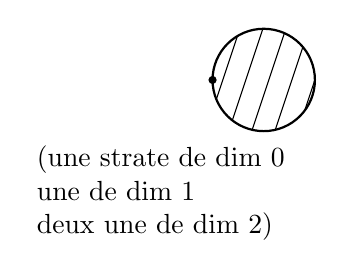
\begin{tikzpicture}[scale=.65]
\begin{scope}\clip (0,0) circle(1);\foreach \x in {-1.2,-.75,-.3,.15,.6}{\draw (\x,-1.2)--(\x+.8,1.2);}\end{scope}
\draw[thick] (0,0) circle(1);\fill (-1,0) circle(.08);
\node[anchor=north east,align=left] at (.6,-1.1) {(une strate de dim 0\\une de dim 1\\\deleted{\unsure{deux}} \inserted{une} de dim 2)};
\end{tikzpicture}}).
Plus précisément encore, on veut ceci:

e) $\forall X_i$, la structure locale autour des $X_i$ \inserted{\unsure{de l'ens.}} des $\overline{X_j}$ tels que $\overline{X_j}\supset X_i$ est \deleted{loc.}

\margin{180}

\scanpage{182}

isomorphe à une structure produit,
\[
X_i\times Z
\]
(avec les $X_j$ correspondant à des $Z_j\subset Z$, $\overline{X_j}$ à $\overline{Z_j}$, $X_i$ à un $z_0\in Z$ contenu dans les $\overline{Z_j}$), et les $\pi_0(Z_j;\overline{Z_j},z_0)$ sont de cardinal 1, i.e. il existe \deleted{\unsure{touj}} un syst. fond. de voisinages de $z_0$ dans $Z$ dont l'intersection avec les $Z_j$ est connexe)

\margin{\uline{NB} les $Z_j$ loc. connexes}

\uline{Remarque:} Si $U$ est un ouvert de $X$, alors l'ens des composantes connexes des $U\cap X_i$ forme \inserted{encore} une stratification \inserted{globale} de $U$. Donc \deleted{l'application} \inserted{pour un} ouvert $U$ variable de $X$,
\[
U\unsure{\mapsto}\mathrm{Strat}_{\mathrm{glob}}(U)
\]
forme un préfaisceau sur $X$. Les exemples de d) montrent que ce préfaisceau n'est pas \deleted{\unsure{séparé}} \inserted{un faisceau} (contre exemple encore plus simple: les feuilletages!)

\margin{j'ai l'impression cependant qu'une stratification globale \unsure{est connue quand on la connaît localement}.}

Les sections du faisceau associé s'appellent les \inserted{\uline{structures de}} \uline{stratification locale} sur $X$. \unsure{Comparer} avec l'exercice de SGA (théorie des Topos) sur les relations d'équivalence locales --- les stratifications en sont des exemples très

\margin{181}

\scanpage{183}
\mspage{87}

particuliers.

\deleted{Sauf erreur}

On suppose donné sur $X$ une structure de stratification locale. Sauf erreur, on peut (comme dans le cas des feuilletages, plus gén. de ttes les relations d'équivalence locales) définir \deleted{l'espace \inserted{déployé de} des feuilles, que je vais} une partition de $X$ en des \deleted{\uline{feuilles}} \inserted{strates}, chaque \deleted{feuille $\unsure{F}$} \inserted{strate $\unsure{E}$} étant munie d'une topologie (qui n'est pas en général la topologie induite) telle que l'inclusion

(296)\quad\diagram{\begin{tikzcd}[ampersand replacement=\&]\unsure{E}\arrow[r]\&X\end{tikzcd}}

soit une immersion locale. Je vais désigner par $D_{\Delta_0}^{*}$ \deleted{la réunion} \inserted{l'espace} somme des feuilles, donc

(297)\quad\diagram{\begin{tikzcd}[ampersand replacement=\&]D_{\Delta_0}^{*}\arrow[r]\&X\end{tikzcd}},

\deleted{\unsure{qui}} est bijective, et une imm. loc.

\margin{182}

\scanpage{184}

\uline{Remarques} a) Si $X$ est compact, on voit qu'il n'y a qu'un nb fini de \deleted{feuilles} \inserted{strates} (qui sont loc. compactes) --- on s'intéresse surtout aux \deleted{feuilletages} \inserted{stratifications} avec un nb fini de strates --- mais bien sûr cette hyp. n'est pas stable par passage à un ouvert de $X$.

b) La formation de $D_{\Delta_0}^{*}$ au dessus de $X$ commute à la restriction à un ouvert de $X$.

c) Si la \deleted{\unsure{partition}} \inserted{structure} de \unsure{strat.} est définie par un diviseur à croisements normaux sur un espace analytique, alors on a un homéo.
\[
(298)\qquad D_{\Delta_0}^{*}\simeq\coprod_{d\in\mathbb N}D_d^{*}
\]
donc la notation $D_{\Delta_0}^{*}$ introduite ici coïncide avec celle des \deleted{\unsure{la}} deux sections précédentes.

\margin{183}

\scanpage{185}
\mspage{88}
\margin{\deleted{\unsure{loc.}}}

On appelle \uline{drapeau} de longueur $r\in\mathbb N$ d'une stratification globale tout système
\[
(299)\qquad \Sigma_*=\{\overline{X_{i_0}}\subset\overline{X_{i_1}}\ \cdots\ \subset\overline{X_{i_r}}\}
\]
de strates --- le drapeau est \uline{non dégénéré} si les inclusions sont strictes.
Un \uline{drapeau local} \inserted{\uline{strict}} de longueur $r$ est un \deleted{système} couple formé d'un tel drapeau, et d'une ``origine'' \deleted{$x\in X_{i_0}$ \uline{NB}.}
\[
(300)\qquad x\in X_{i_0}
\]
\margin{NB on exige $x\in X_{i_0}$ et non seulement $x\in\overline{X_{i_0}}$}

\deleted{On met une topologie sur l'ens des drapeaux de type donné, ou \unsure{ces} drapeaux}
On met une topologie sur l'ens des \uline{drapeaux} \inserted{\uline{locaux stricts}} de \deleted{type} longueur $r$, en prenant comme \deleted{voisinages de $(x,\overline{\Sigma}_*)$} \inserted{\unsure{base d'ouvert|base d'ouverts}} les ensembles qu'on obtient en prenant $\Sigma_*$ fixe, et $x$ variable dans un ouvert de $\unsure{\Sigma_0|\Sigma_*}$.
On trouve un espace topologique $D_{\Delta_{\unsure{r}}}^{*}$, qui s'envoie dans $X$ par

\margin{184}

\scanpage{186}

$(x,\overline{\Sigma}_*)\longmapsto x$, d'où

(301)\quad\diagram{\begin{tikzcd}[ampersand replacement=\&]D_{\Delta_r}^{*}\arrow[r]\&X\end{tikzcd}}

\margin{les images des composantes connexes de $D_{\Delta_r}^{*}$ sont des strates}

qui est une immersion locale. En fait, cet espace sur $X$ ne dépend que de la \inserted{structure de} stratification locale sur $X$ définie par la stratification globale --- on aurait pu le définir directement en termes de la structure locale, à l'aide de la notion de ``drapeaux en germes de strates''. \deleted{Une autre façon de procéder serait de}

\deleted{On aura} \inserted{Dans} le cas d'une stratification associée à un diviseur à cr. norm. sur un esp. analytique, on retrouve les ouverts déjà notés
\[
D_{\Delta_r}^{*}=\coprod_{\substack{\deleted{\unsure{d_*}}\\\unsure{d_r|d_*}\,\unsure{\subset|\in}\,\mathcal P_{r+1}(\mathbb N)}}D_{\unsure{d_r|d_*}}^{*}
\]
de $D_{\Delta_r}$ des deux sections précédentes.

Mais il faudrait pouvoir définir l'analogue des morphismes $\unsure{\tfrac12}$ \unsure{simpliciaux}

\margin{185}

\scanpage{187}
\mspage{89}

\diagram{\begin{tikzcd}[ampersand replacement=\&]D_{\Delta_r}^{*}\arrow[r]\&D_{\Delta_{r'}}\end{tikzcd}}
pour
\diagram{\begin{tikzcd}[ampersand replacement=\&]\Delta_{r'}\arrow[r]\&\Delta_r\end{tikzcd}}
et pour ceci, on \deleted{doit} \inserted{\unsure{penserait à}} définir quelque chose qui tienne lieu de $D_{\Delta_{r'}}$ ---

On va définir les drapeaux pointés \deleted{généraux} \inserted{(pas stricts)} comme étant les systèmes $(x,\overline{\Sigma}_*)$, avec cette fois-ci \unsure{seult}
\[
x\in\overline{X_i}
\]
on définit la topologie comme précédemment, on trouve un $D_{\Delta_r}$ et

(302)\quad\diagram{\begin{tikzcd}[ampersand replacement=\&]D_{\Delta_r}\arrow[r]\&X\end{tikzcd}}

qui est encore une immersion locale, et $D_{\Delta_r}^{*}$ est un ouvert canonique de $D_{\Delta_r}$.

Cette fois-ci on a fait ce qu'il fallait pour que les $D_{\Delta_r}$ forment un système $\unsure{\tfrac12}$ simplicial d'espaces --- les morphismes de dégénérescence fournissant des iso.

Cet espace $\unsure{\tfrac12}$ simplicial est-il

\margin{186}

\scanpage{188}

une catégorie dans $(\mathrm{Top})$? Oui, en d'autres termes, l'application canonique
\[
(303)\qquad D_{\Delta_2}\xrightarrow{\sim}D_{\Delta_1}\mathbin{\times}_{D_{\Delta_0}}D_{\Delta_1}
\]
est iso --- cela exprime simplement que la donnée d'un drapeau \inserted{local} de longueur $2$
\[
\deleted{\unsure{D}}\quad \Sigma_* = \{x\in\overline X_{i_0}\subset\overline X_{i_1}\subset\overline X_{i_2}\}
\]
revient à la donnée de $\{x\in\overline X_{i_0}\subset\overline X_{i_1}\}$ et $\{x\in\overline X'_{j_0}\subset\overline X'_{j_1}\}$ tels que $\overline X_{i_1}=\overline X'_{j_0}$ (il s'agit de germes autour de $x$...)

Donc une \uline{stratification locale} définit une ``catégorie topologique''
\diagram{
\[
(303)\quad\left\{
\begin{array}{l}
\text{espace des objets} = D_{\Delta_0} \\
\hspace{5em}=\text{espace des strates locales}\\
\hspace{7em}\deleted{\unsure{s}}\ \text{pas strictes}\\[.8em]
\text{espace des flèches} = D_{\Delta_1}\\
\hspace{5em}=\text{espace des drapeaux}\\
\hspace{7em}x\in\overline X_{i_0}\subset\overline X_{i_1}\\[.8em]
\text{\uline{morphismes} ``source'', ``but'', ``\unsure{composition|multiplication}''}\\
\hspace{4em}\text{définis de façon évidente}
\end{array}\right.
\]
}

\margin{187}

\scanpage{189}
\mspage{90}

On a ceci:
\[
(304)\qquad D_{\Delta_r}\xrightarrow{\sigma}D_{\Delta_0}
\]
application simpliciale correspondant au ``premier sommet'' d'un simplexe \unsure{ordonné}, ou à la ``source'' d'une suite de flèches
\diagram{\begin{tikzcd}[ampersand replacement=\&,column sep=small]
\bullet \arrow[r,dash] \& \bullet \arrow[r] \& \bullet \arrow[r] \& \cdots \arrow[r] \& \bullet
\end{tikzcd}}

\margin{\uline{NB} $D^*_{\Delta_r}$ est l'image inverse de $D^*_{\Delta_0}$}

\unsure{est} une application finie étale \uline{au dessus} de $D^*_{\Delta_0}$ (\uline{NB} Dans le cas ``croise-ments normaux, c'est $=$ un \unsure{rev.} étale fini sur $D_{\Delta_0}$ tt entier --- mais c'est là un fait très spécial, de $=$ que le fait que les \deleted{\unsure{diff.}} strates \unsure{soient} des variétés topologiques --- ce qui implique \unsure{donc} qu'il en est \unsure{donc|bien} de $=$ des $D_{\Delta_{\unsure{*}}}$.)

Egalement le fait que \deleted{\unsure{la}} la structure ordonnée \inserted{locale} de $D^*_{\Delta_{\unsure{*|1}}}$ sur $D^*_{\Delta_0}$ (\deleted{flèches} structure \inserted{de l'ens.} des strates locales contenant une strate locale donnée) soit \deleted{\unsure{une|celle d'une}} \inserted{isomorphe} \deleted{structure de simplexe}

\margin{188}

\scanpage{190}

à l'ens des parties d'un ens. fini, est spécial \unsure{aux} croisements normaux ce n'est déjà plus le cas pour
\figure{\begin{tikzpicture}[baseline=-.3ex,scale=.9]
\draw (0.02,.09) -- (.18,.69);
\draw (-.10,-.05) to[out=200,in=15] (-.56,-.21);
\draw (.10,-.06) -- (.48,-.25);
\draw (0,0) circle[radius=.035];
\end{tikzpicture}}, où le nb des strates contenant $\bullet$ est (en comptant $\bullet$ lui-$=$) de $7$, qui n'est pas une puissance de deux...

\uline{NB} Pour l'instant, on n'a pas fait usage de l'hypothèse \inserted{\unsure{du moins|des voisinages}} de locale trivialité de p.\ 86 e). Elle servira plus loin, pour expliciter en termes de fibrations loc.\ triviales certains voisinages tubulaires, \deleted{qui \unsure{seront à l'origine}} \inserted{jouant le rôle} des ``topos élémentaires'' de la section précédente.

\margin{189}
